% this file is called up by thesis.tex
% content in this file will be fed into the main document

%------------------------------------------------------------------------- 

\chapter{Generación de Vórtices Ópticos}
\label{cha:Gen_intro}

\graphicspath{{Figures/ch2_img/}{../Figures/ch2_img/}}
\lhead{Generación de Vórtices Ópticos: \textit{Introducción}} % This is for the header on each page - perhaps a shortened title

\section{Estado del Arte} %Introducción????
\label{sec:ChGen_estado_del_arte}
\lhead{Generación de Vórtices Ópticos: \textit{Estado
    del Arte}}
Los haces con OAM distinto de cero inicialmente fueron generados en el
laboratorio por medio de técnicas analógicas entre las que se destacan
el uso de conversores modales \citepChGen{Alekseev1998}, placas de fase espiral grabadas en sustratos
transparentes \citepChGen{Jun2009}, y hologramas de fase impresos en acetato
\citepChGen{Carpentier2008} . La conversión modal utiliza sucesiones de
lentes astigmáticas para convertir los modos Hermite Gauss en modos
Laguerre Gauss, y fue la primera forma en la cual se produjeron VO en
el laboratorio. A diferencia de la conversión modal, - que requiere un
montaje experimental muy sensible a desplazamientos -  las técnicas que utilizan máscaras
de fase se caracterizan por necesitar sólo un elemento óptico que
permite modificar punto a punto la fase de un haz que originalmente
carecía de momento angular, para convertirlo en un haz con vorticidad
óptica. El uso de placas físicas grabadas con un patrón espiral
tiene la ventaja de generar haces LG con sólo ubicarlas en
el camino óptico del haz, y tiene la desventaja de que una vez
fabricadas no se pueden modificar. 
En situaciones donde es requerido generar haces del tipo LG con la suficiente
flexibilidad como para corregir aberraciones ópticas, se
necesita de dispositivos digitales con propiedades similares a los
dispositivos analógicos mencionados anteriormente. Estos dispositivos
se conocen como moduladores espaciales de luz o SLM por sus siglas en
inglés. En este proyecto se pretende generar VO y caracterizar su
frente de onda utilizando un tipo de SLM's que modifican la fase de la
luz cuando ésta pasa a través de ellos. 

\subsection{Moduladores Espaciales de Luz}

Como su nombre lo indica, los moduladores espaciales de luz sirven
para modular punto a punto las propiedades de la luz sobre un
plano. Ya sea solamente su amplitud como en los dispositivos de
visualización de cristal líquido (pantallas LCD), o su fase, como en
los dispositivos que se ilustran en la figura \ref{fig:LCDSLM}.
\begin{figure}[h!]
\centering
    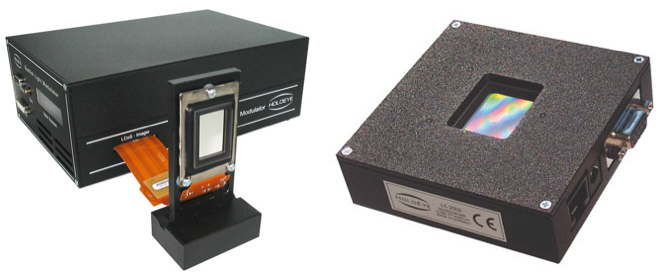
\includegraphics[width=0.5\textwidth]{LCDSLM.png}
\caption[Comparación entre TN-SLM]{Moduladores espaciales modelo PLUTO y LC2012 de reflexión y
  transmisión marca Holoeye basados en la tecnología de cristal
  líquido. Por ser fabricado a partir de un LCD comercial el modulador de
  la derecha es ensamblado a una cuarta parte del costo del izquierdo.}
\label{fig:LCDSLM}
\end{figure}

Si diferenciamos los SLM por el tipo de tecnología, estos pueden ser
agrupados en dos categorías: basados en cristales líquidos, o en
arreglos de micro espejos (figura \ref{fig:MEMSLM}), mejor 
conocidos en la industria de la proyección como DLP (de Digital Light
Processing).  
\subsubsection{Moduladores basados en micro espejos}
En su mayoría, los moduladores comerciales basados en arreglos de micro
espejos funcionan con micro mecanismos que inclinan una superficie
reflectiva de tal forma que se modifique la cantidad de luz que un
observador ve desde una perspectiva dada, es decir que modulan
intensidad. Sin embargo, con el interés de modular fase además de
intensidad se han desarrollado nuevos micro mecanismos que
permiten desplazar verticalmente el espejo sin modificar su
inclinación, introduciendo así un cambio en la distancia del camino
óptico y por ende, la fase tal y como se presenta en los trabajos de
\citetChGen{Wu2010} y \citetChGen{Liesener2006}. Dado que es una
tecnología incipiente y ha tenido menor tiempo en el mercado que los
cristales líquidos, estos sistemas y en particular los de tipo pistón,
siguen teniendo precios elevados y aún están lejos de ser utilizados
en muchos laboratorios. 
\begin{figure}[h!]
\centering
    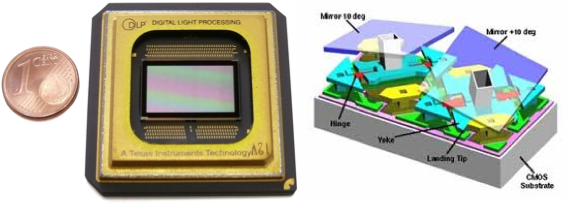
\includegraphics[width=0.5\textwidth]{MEMSLM.png}
\caption[Modulador espacial basado en arreglos de micro espejos]{Modulador espacial basado en arreglos de micro espejos marca Texas Instruments.}
\label{fig:MEMSLM}
\end{figure}

\subsubsection{Moduladores de cristal líquido}
Los SLM basados en Cristales Líquidos (LCs) aprovechan las propiedades
físicas de ciertos polímeros que dada su forma alargada y propiedades
electrónicas polares, cambian su orientación ante la presencia de
campos eléctricos.  Esta sensibilidad a los campos eléctricos, en
conjunto con sus propiedades ópticas anisotrópicas permitió que desde
los años 70s se implementaran LCs para generar imágenes en pantallas de
dispositivos como relojes, calculadoras y luego televisores y
proyectores. Fue más adelante cuando estudios especializados de las
propiedades de los LCs como los realizados por
\citetChGen{Yeh1999} y \citetChGen{Yariv2002}, y experimentos como los de
\citetChGen{Konforti1988} demostraron que los LCD pueden ser usados
como moduladores de solo fase. Aunque la aplicación de LCs para
modulación de fase es relativamente reciente, el estudio de sus
propiedades físicas no lo es y desde los años 60’s la investigación ha
sido respaldada por grandes empresas interesadas en desarrollar
productos tecnológicos de generación y procesamiento de imágenes como
RTC, Hamamatsu, Hitachi, HP, Texas Instruments, Sony y otros. Dado
el interés por entender los LC, se ha llegado a modelos matemáticos y  técnicas de  
caracterización robustas que permiten extraer los parámetros de un SLM para
 simular su comportamiento. 
El desarrollo de estas técnicas ha permitido a investigadores 
alrededor del mundo implementar moduladores de fase a
partir de elementos LCD extraídos de dispositivos de proyección
comerciales, entre ellos se encuentran los trabajos de
\citepChGen{Pezzaniti1993,Soutar1994,Zhang1994,Moreno1998,Davis1999,Iemmi2001,Davis2003,Moreno2003,Kim2005,Duran2006,Duran2007,Marquez2007,Liu2010,Ma2010,Ma2011,Yu2012}. Mientras
que autores como Mahmud, \citepChGen{Mahmud2008}, Roopahsree
\citepChGen{Roopashree2009a}, y David \citepChGen{Dev2012}
caracterizaron un Holoeye LC2002 que es vendido comercialmente como
modulador de amplitud y fase.
Ejemplo de la práctica de reensamblar un LCD y venderlo como SLM es el
modulador marca Holoeye LC2012 que gracias a usar un LCD comercial
marca Sony es ensamblado a una cuarta parte del precio de otros
moduladores. 

Adicionalmente, cabe mencionar que los moduladores en base a LC se
dividen en dos tipos, de reflexión y de transmisión. Sin entrar en
detalle, los primeros permiten modulaciones de fase que van hasta $2\pi$
radianes, tienen mayor resolución, necesitan menos elementos de
polarización para su uso, tienen altas velocidades de operación y el
hecho de que la electrónica esté detrás del cristal (y detrás de la
superficie reflectiva) hace que se produzcan menos efectos indeseados
de difracción. Todo esto a costa de desarrollar LCs y
electrónica personalizados. En cambio, los moduladores de transmisión
se ensamblan a partir de LCs comerciales que fuera de polarizar la luz
retardan su fase. Esto implica un acople entre modulación de fase y 
modulación de intensidad que se traduce en menor calidad de la
modulación de fase total. Para lograr una modulación específica se
necesitan polarizadores y retardadores que generen un 
estado de polarización particular a la entrada del SLM. Por otra
parte, al tener la electrónica acoplada sobre el cristal y no en un
elemento separado como en los de reflexión, se limita la
resolución; no todo el volumen de LC se aprovecha y se introducen
efectos indeseados de difracción. 
No obstante, los SLM de transmisión son muy económicos y algunos
autores como Davis et al. \citepChGen{Davis2000, Davis2013} han propuesto
que se podrían usar como dispositivos para modular polarización. En
base a la idea de usarlos para modular polarización, otros como \citetChGen{Moreno2004, Moreno2011} han
combinado el formalismo de Fourier con el de las matrices de Jones
para modelar el comportamiento de dispositivos ópticos de Fourier que
involucran polarización. 

En el laboratorio de metrología óptica del grupo de Óptica Aplicada de
la Universidad EAFIT se encuentran dos moduladores de transmisión
marca Holoeye modelos LC-2002 y LC- 2012 que en el contexto de este
trabajo han sido caracterizados para optimizar su uso en aplicaciones metrológicas
tales como la creación y corrección de aberraciones en haces LG.  
La generación de VO se da entonces una vez se tenga apropiada la
herramienta que los produce.  
A lo largo de este capítulo se presentarán los conceptos teóricos
necesarios para entender la caracterización de SLMs y luego se
presentarán las diversas herramientas y métodos que se implementaron
para lograr la generación de VO.

% En la sección que sige se introduce la segunda mitad del
% problema, es decir, ¿Cómo caracterizar y corregir las aberraciones ópticas de un VO?

% \subsection{Aberraciones ópticas}

% Los VO generados en el laboratorio están sujetos a aberraciones
% ópticas que se asocian a situaciones tales como:
% \begin{itemize}
% \item Problemas en la alineación de componentes ópticos como
%   lentes o espejos.
% \item Deformaciones en las superficies de elementos como
%   polarizadores, lentes, espejos, láminas retardadoras, e incluso de
%   las céldas de cristal líquido en el SLM.
% \item Presencia de partículas de polvo en las superficies de las
%   componentes ópticas que inducen efectos indeseados de difracción. 
% \end{itemize}

% Adicionalmente, y siguiendo con el tema de la sección anterior, los
% SLM de transmisión basados en pantallas de LC introducen otras fuentes
% de aberraciones. En primera medida, los LCD son dispositivos discretos en dos de los
% sentidos de la palabra; por un lado, son discretos espacialmente y
% las señales de control son asignadas a subdivisiones del cristal de tamaño finito
% conocidas como píxeles. El arreglo rectangular de todos los píxeles
% genera efectos de difracción similares a los de rejillas verticales y
% horizontales combinadas. Esto quiere decir que el SLM separa los
% órdenes de difracción de la luz que pasa a travez de él. Asimismo, el
% hecho de ser una cuadrícula discreta hace que el modulador no pueda
% generar distribuciones de fase en regiones infinitamente pequeñas como
% sería deseado alrededor de una singularidad óptica. Como ejemplo, en la figura
% \ref{fig:discrete_mask} a) se muestra una imagen de la región donde
% resultaría una singularidad óptica en una máscara de
% fase espiral enviada al SLM. Como se puede ver, la máscara de fase
% discreta resulta muy distinta a la máscara ideal presentada en la
% figura \ref{fig:oam_intro}b), y por lo tanto introduce deformaciones
% en el haz Laguerre-Gauss que resulta a la salida del SLM.   

% \begin{figure}[h!]
% \centering
% 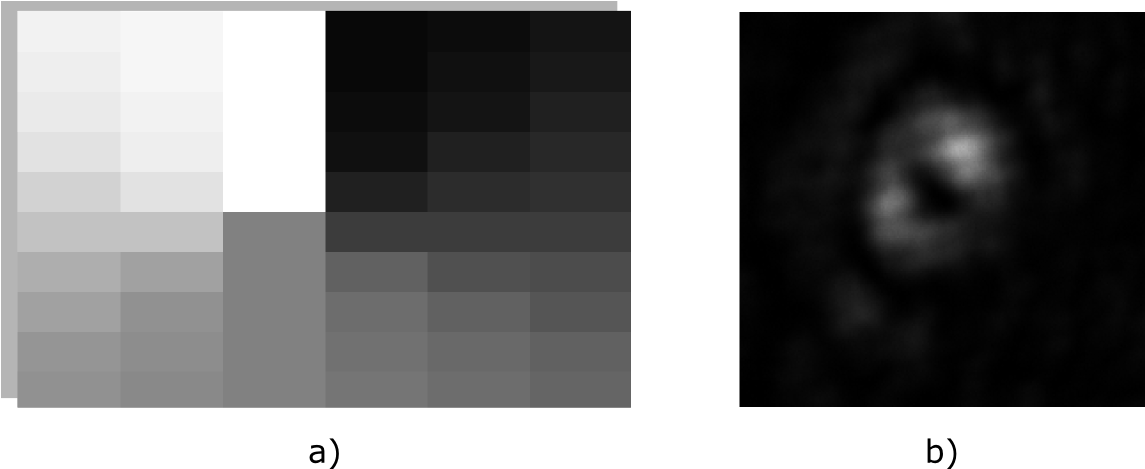
\includegraphics[ scale=.4]{discrete_mask.png}
% %Las imagenes que enviamos al SLM son generadas en un
% %  ordenador que de por sí es discreto, y llegan a un dispositivo
%  % físico que tiene divisiones discretas, tanto espaciales como
%  % electrónicas. Aún 
% \caption[Efecto de pixelado eb el SLM sobre las aberraciones en VO]{a) Magnificación de una mascara tipica proyectada al SLM. b) Imagen de un VO de poca calidad producido con un SLM de
% transmisión modelo Holoeye LC2002.}
% \label{fig:discrete_mask}
% \end{figure}

% Por otra parte, el SLM es discreto en la medida que sólo puede asignar
% níveles de voltaje discretos (0-255 divisiónes de 5V) a cada una de
% las celdas. Este fenómeno también es observable en la figura
% \ref{fig:discrete_mask}a) y puede introducir efectos
% indeseados. Más aún, si cómo el nuestro, el modulador no llega a una
% modulación de sólo fase, o tiene una modulación que no llega a
% completar el ciclo de $2\pi$ radianes. 
% Todas las posibles fuentes de error mencionadas anteriormente se
% combinan para generar haces Laguerre-Gauss de poca calidad como el que se muestra
% en la figura \ref{fig:discrete_mask} b). 


\section{Marco Teórico de la Caracterización de SLMs de Trasmisión}
\label{sec:ChGen_marco_teorico}
\lhead{Generación de Vórtices Ópticos: \textit{Marco Teórico}}

Dado que los SLMs de transmisión se ensamblan a partir de LCs, lo
primero que hay que tener en cuenta para su caracterización 
es conocer sus generalidades y entender sus propiedades ópticas. 
Entenderemos que los LCs afectan el estado de polarización de la luz y
por ello se dedicará un espacio del marco teórico a presentar los conceptos
generales y herramientas matemáticas propias de la teoría de polarización. 
Una vez presentadas estas herramientas se mostrarán los modelos
actuales con los cuales se representa matemáticamente la modulación de
un LC y se hará una breve revisión de la literatura de la
caracterización de SLMs. 

\subsection{Cristales líquidos}
\subsubsection{Características de los LC}  
Un cristal Líquido es una sustancia que posee propiedades que
se asemejan tanto a las de los sólidos cristalinos como a las de los
líquidos, y puede ser visto como un líquido en el cual existe
orden entre sus moléculas. Para ilustrar esta idea recordemos que los
sólidos cristalinos son un estado de la materia que se caracteriza por
su rigidez y fuertes enlaces químicos, en el cual se puede
establecer un orden posicional en todas las direcciones tal y como se
ilustra en la figura \ref{fig:solido}. Esto implica que la posición de
las moléculas o átomos que lo componen puede ser abstraída como una
red periódica que cumple ciertas reglas de simetría. En cambio, un
líquido amorfo como el de la figura \ref{fig:liquido} tiene enlaces
más débiles por lo cual puede fluir y está compuesto
por moléculas que están completamente desorganizadas. 
\begin{figure}[h!]
\centering
\begin{subfigure}{.45\textwidth}
  \centering
  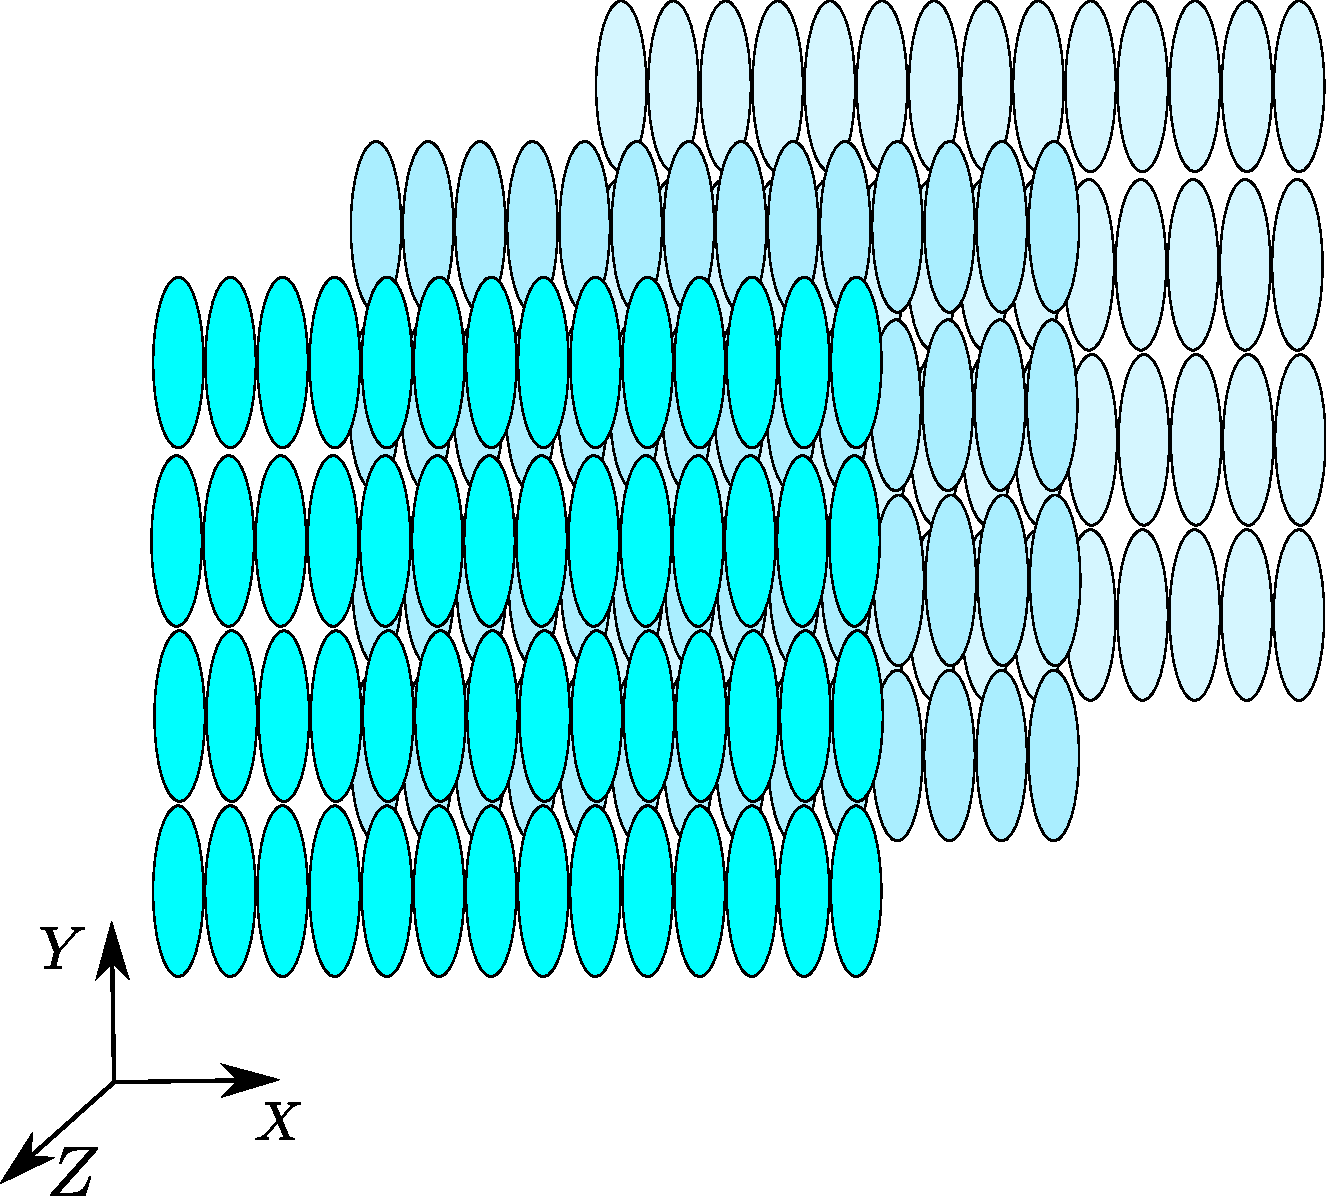
\includegraphics[width=.6\linewidth]{Cristaline_solid}
  \caption{Moléculas con orden posicional y orientacional en un sólido cristalino.}
  \label{fig:solido}
\end{subfigure}\qquad
\begin{subfigure}{.45\textwidth}
  \centering
  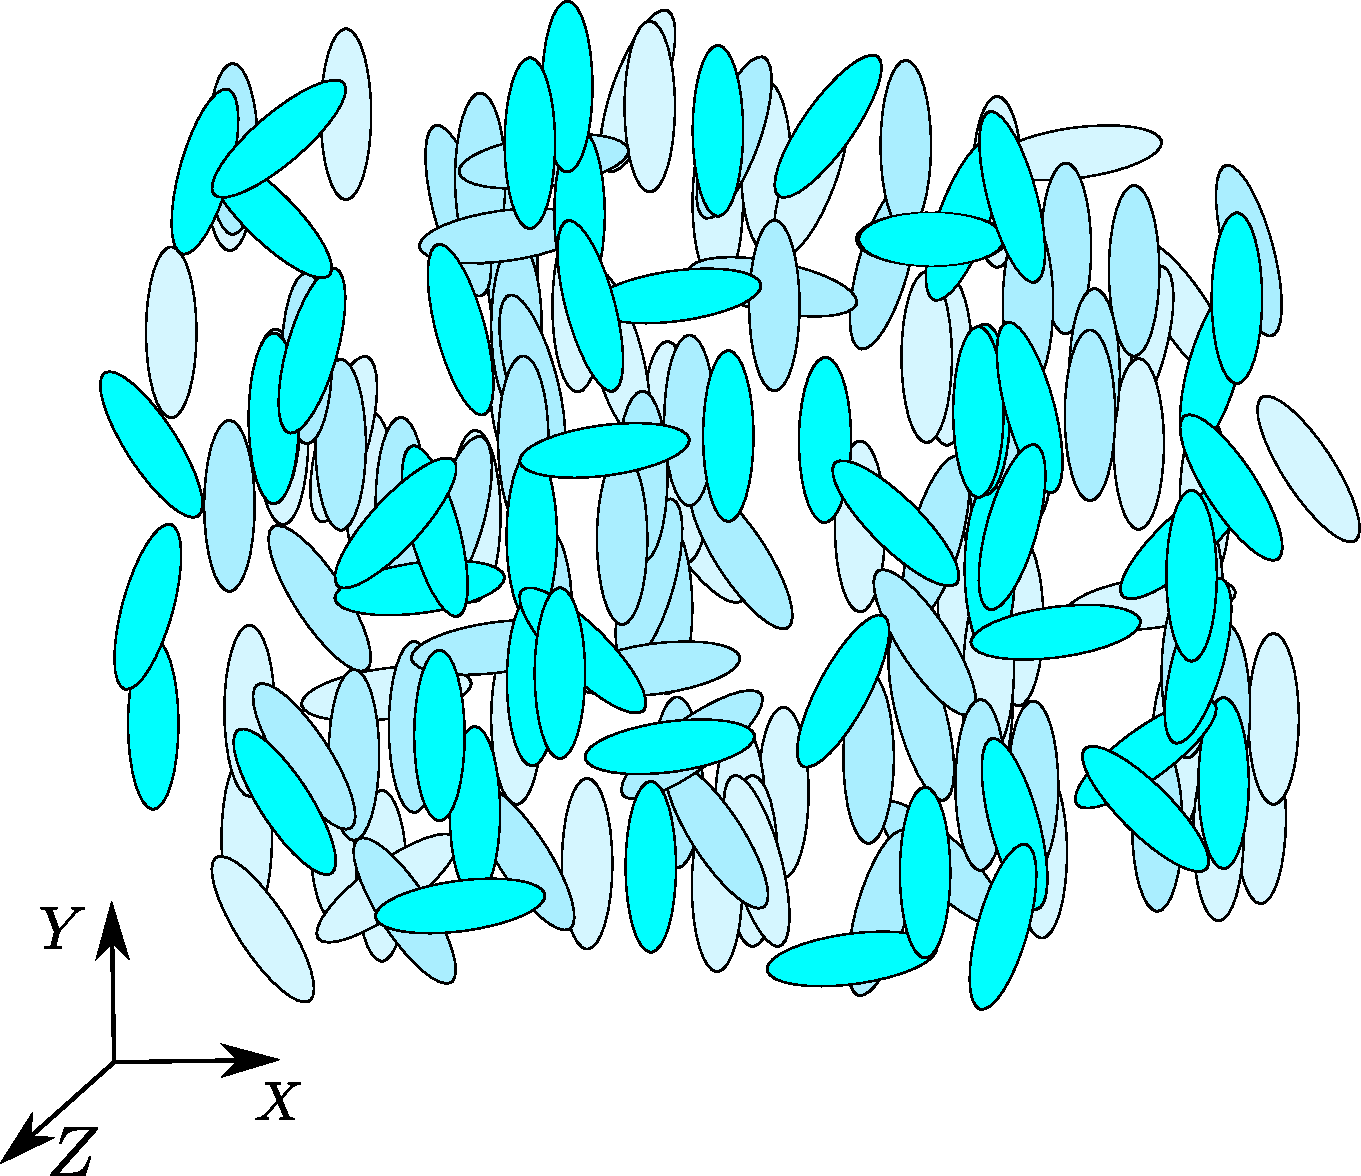
\includegraphics[width=.6\linewidth]{liquid}
  \caption{Moléculas desordenadas pero cercanas en un líquido.}
  \label{fig:liquido}
\end{subfigure}
\caption{Dos estados de la materia comunes en la naturaleza.}
  \label{fig:estados}
\end{figure}

Los cristales líquidos son sustancias que como los
sólidos poseen cierto orden y que pueden fluir como los líquidos. 

Por otra parte, los LCs pueden ser clasificados en tres tipos o fases distintas
conocidas como, \textit{nemáticos},
\textit{smeticos} y \textit{colestéricos}, y más adelante se abordará esta
clasificación. No obstante su diversidad (más de 100.000 compuestos
distintos según \url{http://www.lci-publisher.com}), la característica común de los LC es que están
compuestos de moléculas altamente anisotrópicas, esto es, que sus
propiedades (ópticas, eléctricas y mecánicas) dependen de la
dirección desde la que se observen. La anisotropía se debe tanto a la
geometría alargada o achatada de las moléculas, como a las propiedades
electrónicas de sus componentes.  En el caso de moléculas
alargadas de LCs como la de la figura \ref{fig:LCMolecule} la
estructura química de un LC genéral se
compone de un sistema de anillos aromáticos que pueden ser o no
saturados conectados por un grupo de conexión A, y sujetos a dos
cadenas o grupos terminales X y Y \citepChGen{Yeh1999}. 
\begin{figure}[h!]
\centering
    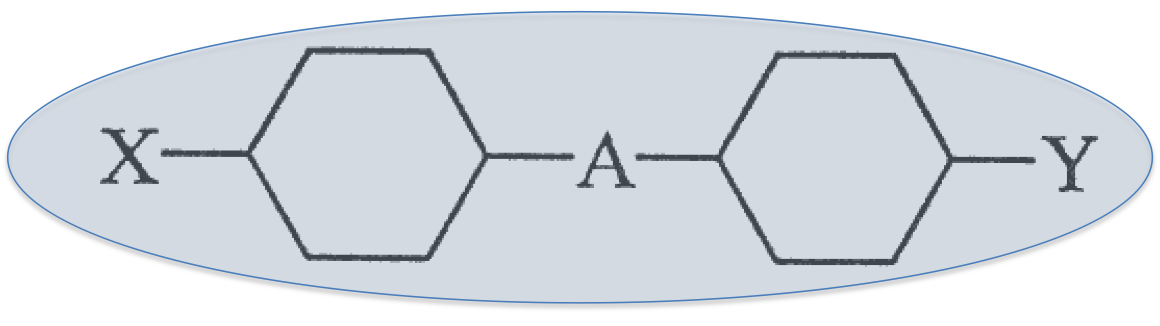
\includegraphics[width=0.5\textwidth]{LCMolecule}
\caption{Esquema de la composición química general en una molécula de LC.}
\label{fig:LCMolecule}
\end{figure}

La presencia de los anillos proporciona las fuerzas intermoleculares de corto alcance que
son necesarias para formar fases nemáticas y el tipo de anillos
(saturado o no saturado) determina la presencia o no de enlaces $\pi$
que se asocian a orbitales $P_z$ de los electrones. Esto a su vez
afecta la absorción en el ultravioleta y la birefringencia; se observa mayor
birefringencia en LC con anillos no saturados y mejor comportamiento
en el ultravioleta para anillos saturados.  Luego, las cadenas del
grupo terminal X pueden ser de tres tipos:
\begin{itemize}
\item Cadenas alquilos (alkyl)  $C_nH_{2n+1}$: 
\item Grupos alcoxy $C_nH_{2n+1}O$
\item Grupos alilos (alkenyl) $CH_2=CH-CH_2-$
\end{itemize}
 La longitud de las cadenas X influencia tanto las constantes elásticas
 como las temperaturas de transición de fase. Para cadenas cortas con
 uno o dos átomos de carbono los grupos son muy cortos como para
 presentar fases de LC. Los grupos terminales de tamaño medio: n = 3-8
 son los más adecuados para para construir fases nemáticas por su
 mayor anisotropía, y los compuestos con cadenas aún más largas
 exhiben fases smeticas. La temperatura a la cual la solución pasa de
 ser nemática a isotrópica se conoce como el punto de aclarado o
 \textit{clearing point}, en términos generales, esta temperatura
 disminuye en la medida en la que se alargan los tamaños del 
 grupo terminal X. La función que relaciona el punto de aclarado con
 el número de átomos de carbono es una función suave en la cual los
 números pares generan temperaturas más bajas que los impares. Fuera
 de esto, las propiedades mecánicas como la viscosidad también se ven
 afectadas por el tamaño de los grupos terminales, cadenas
 largas implican viscosidades más altas, y por ello frecuencias de
 operación más bajas. 
Finalmente, las cadenas que forman el grupo terminal Y son las que
tienen mayor influencia en las constantes dieléctricas de la molécula
($\epsilon_x,\epsilon_y$), y asimismo su anisotropía dieléctrica
$\Delta\epsilon$ variables que como veremos más adelante son las que
determinan la birrefringencia del LC asociada a la modulación de fase.
Las cadenas del grupo terminal Y pueden ser:
\begin{itemize}
\item No polares: No Influencian mucho la anisotropía dieléctrica, un
  ejemplo es el grupo alquilo $CnH2n+1$.
\item Polares:  Como CN, F, y Cl. Su alta polaridad induce en la
  molécula una alta anisotropía dieléctrica y por tanto alta
  birrefringencia. La alta anisotropía se obtiene a costa de alta viscosidad, resistividad
  insuficiente y problemas de estabilidad bajo iluminación 
  ultravioleta. Los grupos Y muy polares como los que contienen
  cianuro CN No son buenos para operar a  altas temperaturas como por
  ejemplo proyectores, y sufren de degradación en el UV. Para esas
  aplicaciones se utilizan compuestos menos polares como el flúor o
  cloro que tienen menor birrefringencia.
\end{itemize}

\subsubsection{Clasificación de los LC}  
\label{sec:LC-clasification}
En 1922 y sintetizando los hallazgos de 30 años desde el descubrimiento
de los LCs, el cristalógrafo George Friedel publicó un artículo \citepChGen{Friedel1922}
en el que clasifica los LC en tres tipos básicos conocidos como
cristales smeticos, nemáticos y colestéricos.
En términos de orden, los LC sméticos son los más similares a un
sólido, y los nemáticos se asemejan más a un líquido, y en la medida
en la que se calienta un LC éste realiza una transición desde cristal
smetico hasta líquido isotrópico pasando por la fase nemática. Los estados
colestéricos son un tipo particular de LC nemáticos que a diferencia
de los anteriores tienen propiedades inhomogeneas. 
La principal característica que le da una medida de orden a los LC es
la tendencia de sus moléculas a orientarse en una dirección
preferente gracias a su distribución polar de cargas. Esta tendencia
se puede observar claramente en las figuras \ref{fig:smetic} y
\ref{fig:nematic} como si las moléculas fueran vagones de un tren que
se siguen uno detrás del otro en forma de hilo \footnote{La palabra
\textit{Nematic} proviene de la expresión griega \textit{nema} que
significa hilo.}.  

La orientación preferencial de las moléculas les
otorga una cierta medida de orden a los LC que en adelante llamaremos orden
orientacional. La \textit{cantidad} de orden se medirá por medio de un
parámetro estadístico conocido como parámetro de orden que relaciona
la orientación de las moléculas individuales con la orientación
preferencial o vector director $\vec{n}$ en las vecindades de
la molécula. Si se tiene un conjunto de moléculas como la que se
ilustra en la figura \ref{fig:angulo_director} dónde 
$\theta$ es el ángulo que se forma entre el eje mayor de la molécula
$\vec{v}$ y el vector director, el parámetro de orden orientacional
del cristal se da como el siguiente promedio estadístico sobre todas
las moléculas.

$$ S = \frac{1}{2}\left<3\cos^2{\theta-1}\right>$$
 
\begin{figure}[h!]
\centering
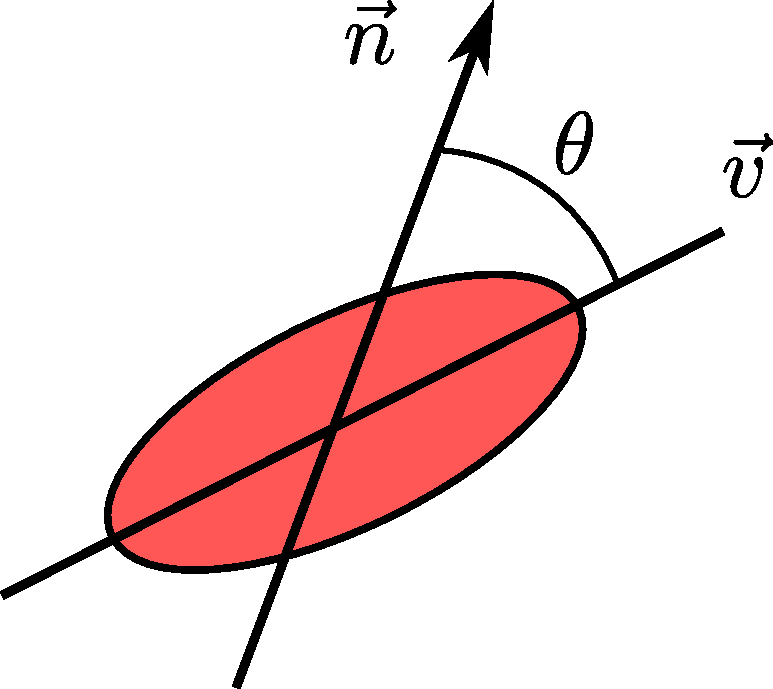
\includegraphics[width=.3\linewidth]{angulo_director}
\caption{Orientación de una molécula de LC con respecto al ángulo
  director en su vecindad.}
\label{fig:angulo_director}
\end{figure}

Un LC con sus moléculas alineadas perfectamente paralelas tiene un
parámetro de orden $S=1$, mientras que un LC con moléculas orientadas
aleatoriamente posee un parámetro $S=0$. El parámetro de orden depende
tanto del tipo de molécula como de la temperatura; en la medida en la
que aumenta la temperatura las moléculas pierden su alineación y el LC
se convierte en un líquido isotrópico. El parámetro de orden gana
importancia cuando se necesita seleccionar un LC que deba ser usado en
rangos de temperatura especiales y se necesite garantizar anisotropía.

\begin{figure}[h!]
\centering
\begin{subfigure}{.4\textwidth}
  \centering
  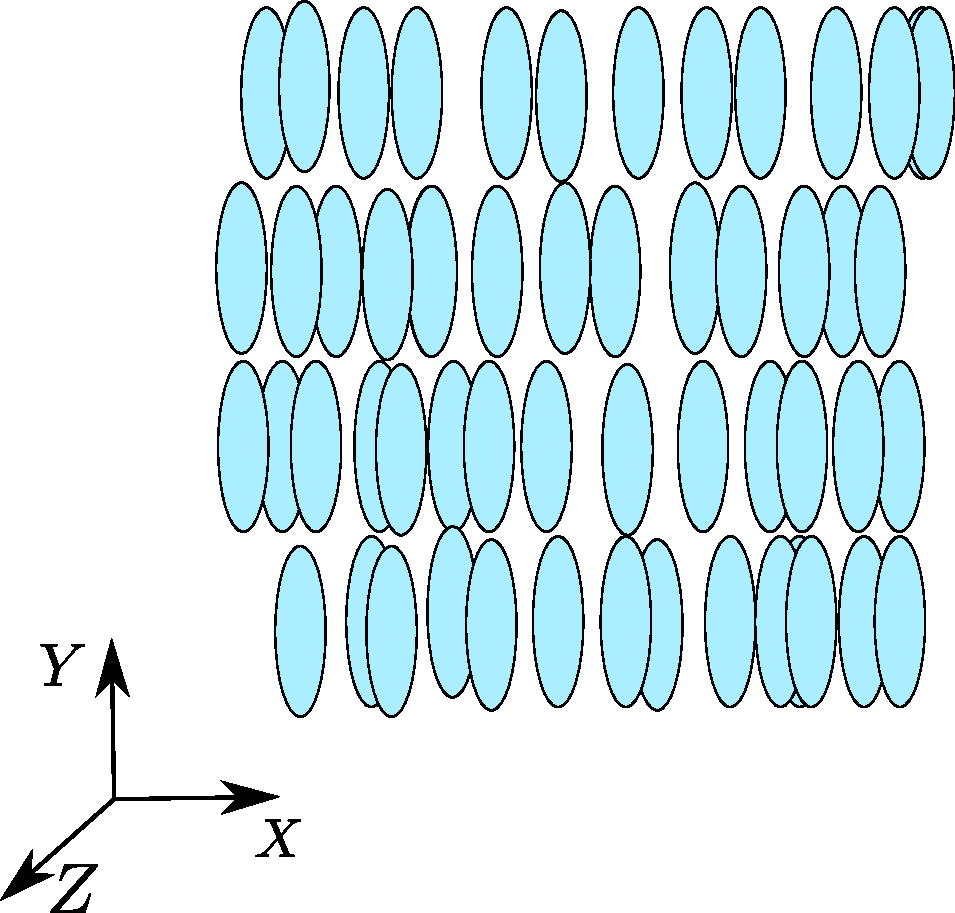
\includegraphics[width=.6\linewidth]{Smetic_LC}
  \caption{Cristal líquido smético.}
  \label{fig:smetic}
\end{subfigure}\qquad
\begin{subfigure}{.4\textwidth}
  \centering
  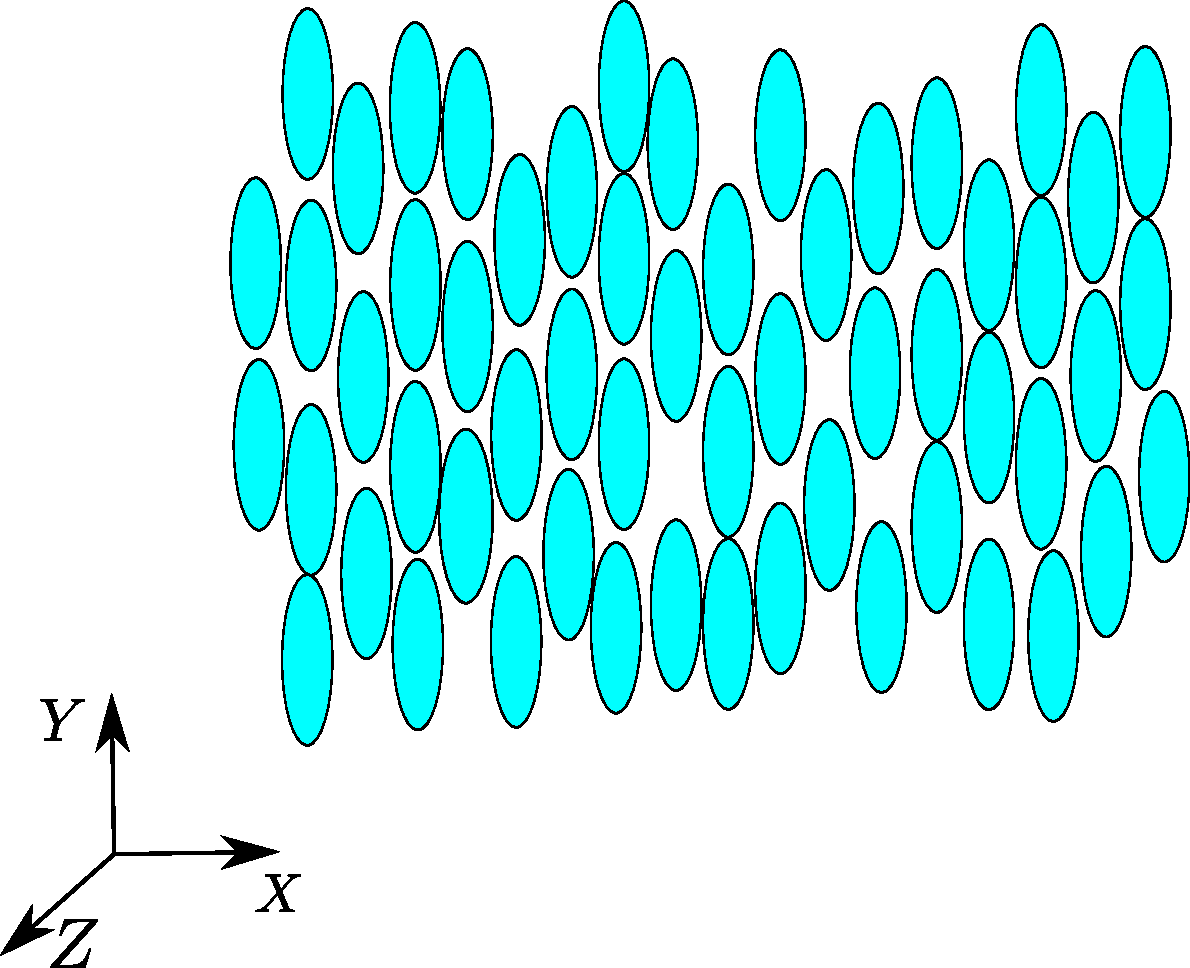
\includegraphics[width=.6\linewidth]{Nematic_LC}
  \caption{Cristal líquido nemático.}
  \label{fig:nematic}
\end{subfigure}\\
\begin{subfigure}{.5\textwidth}
  \centering
  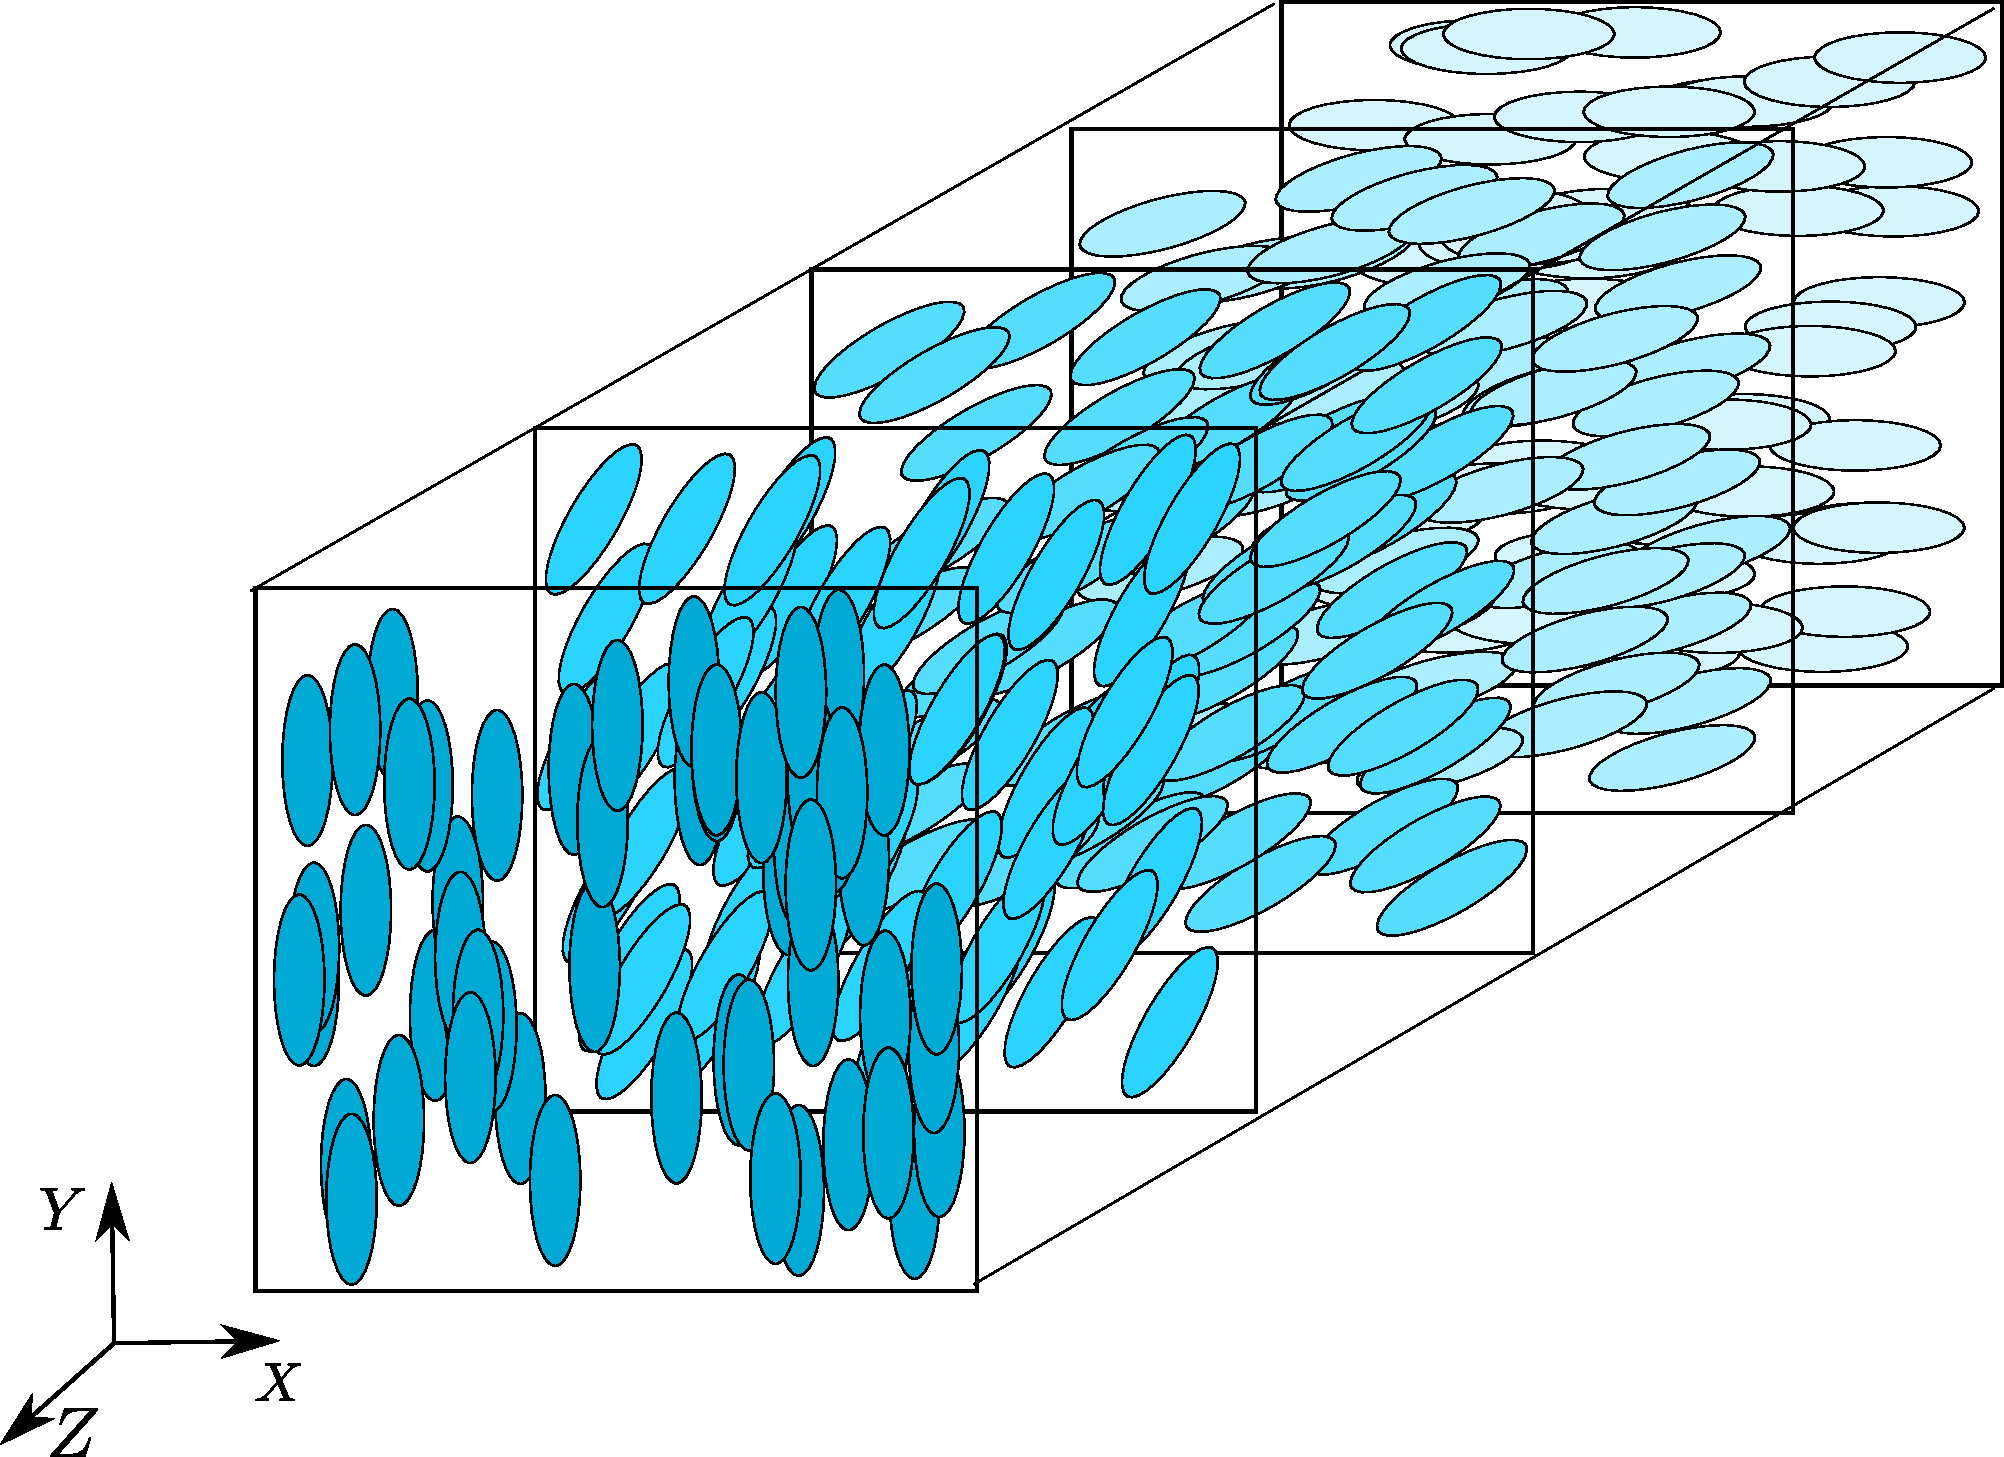
\includegraphics[width=.6\linewidth]{Cholesteric_LC_2}
  \caption{Cristal líquido colestérico.}
  \label{fig:cholesteric}
\end{subfigure}
\caption{Clasificación de los cristales líquidos según su orden.}
\label{fig:CL_clasificacion}
\end{figure}

Los Cristales smeticos como el que se ilustra en la figura
\ref{fig:smetic} se diferencian de los nemáticos en que poseen orden
posicional en una dirección además de orden orientacional. Sin embargo,
este orden viene acompañado de propiedades mecánicas que son menos
convenientes para la construcción de LCDs y por ello las fases
nemáticas y colestéricas son las que tienen mayor número de
aplicaciones en dispositivos electro ópticos. 
A diferencia de las fases smetica y nemática que tienen un solo vector
de orientación, en los cristales líquidos colestéricos el vector
director varía a través del medio de una forma bien
definida y por ello se consideran medios inhomogeneos. Generalmente la
variación es helicoidal como la que se ve en la figura \ref{fig:cholesteric}.   
La variable que caracteriza un cristal líquido colestérico es el
ángulo de inclinación o pitch que forman las moléculas inclinadas con
respecto al eje óptico del material. 


\subsubsection{Las pantallas de cristal líquido nematico retorcido.}


Los moduladores de LC de transmisión que se usan para proyección se
construyen usando una configuración conocida como Twisted
Nematic (TN-LCD) o nematicos retorcidos. Los TN-LCD son
dispositivos como el que se ilustra en la figura \ref{fig:tn-lcd} en
los cuales una  solución de cristal líquido nemático 
se inyecta entre dos superficies rígidas transparentes que han sido frotadas
a lo largo de una dirección preestablecida. Las moléculas del LC en contacto con las
superficies transparentes se adhieren a los canales microscópicos que
resultan del frotado, tomando así su dirección. Cuando las direcciones
de frotado de las superficies en ambos extremos no coinciden, la
dirección preferente de orientación de las moléculas cambia
gradualmente en profundidad desde la dirección del plano de entrada hasta la del
plano de salida como se ve en la figura
\ref{fig:tn-lc}.  El resultado es un cristal líquido inhomogeneo
parecido a un cristal colestérico en el cual la orientación de las
moléculas varía de forma lineal.

\begin{figure}[h!]
\centering
\begin{subfigure}{.45\textwidth}
  \centering
  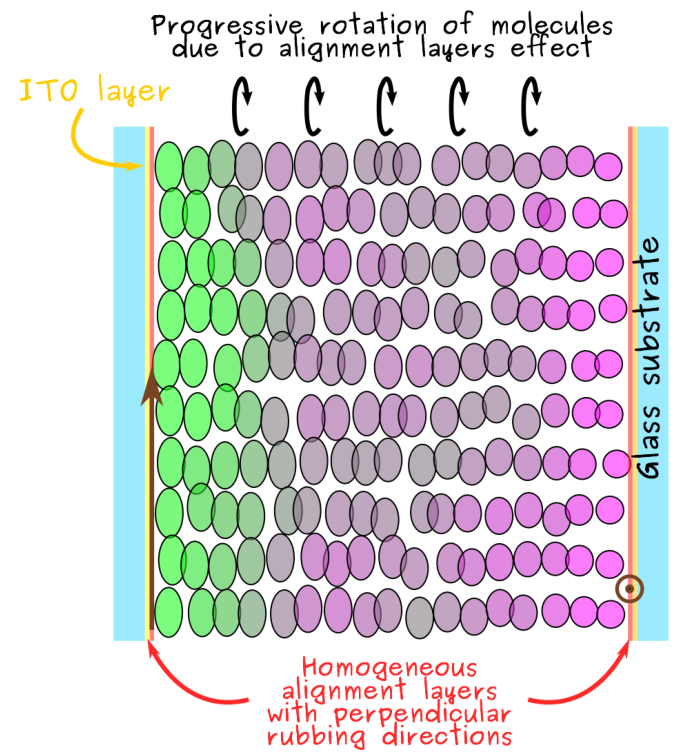
\includegraphics[width=.8\linewidth]{tn-lcd}
  \caption{Esquema de un TN-LCD cuando no hay un voltaje entre las placas.}
  \label{fig:tn-lc}
\end{subfigure}\qquad
\begin{subfigure}{.45\textwidth}
  \centering
  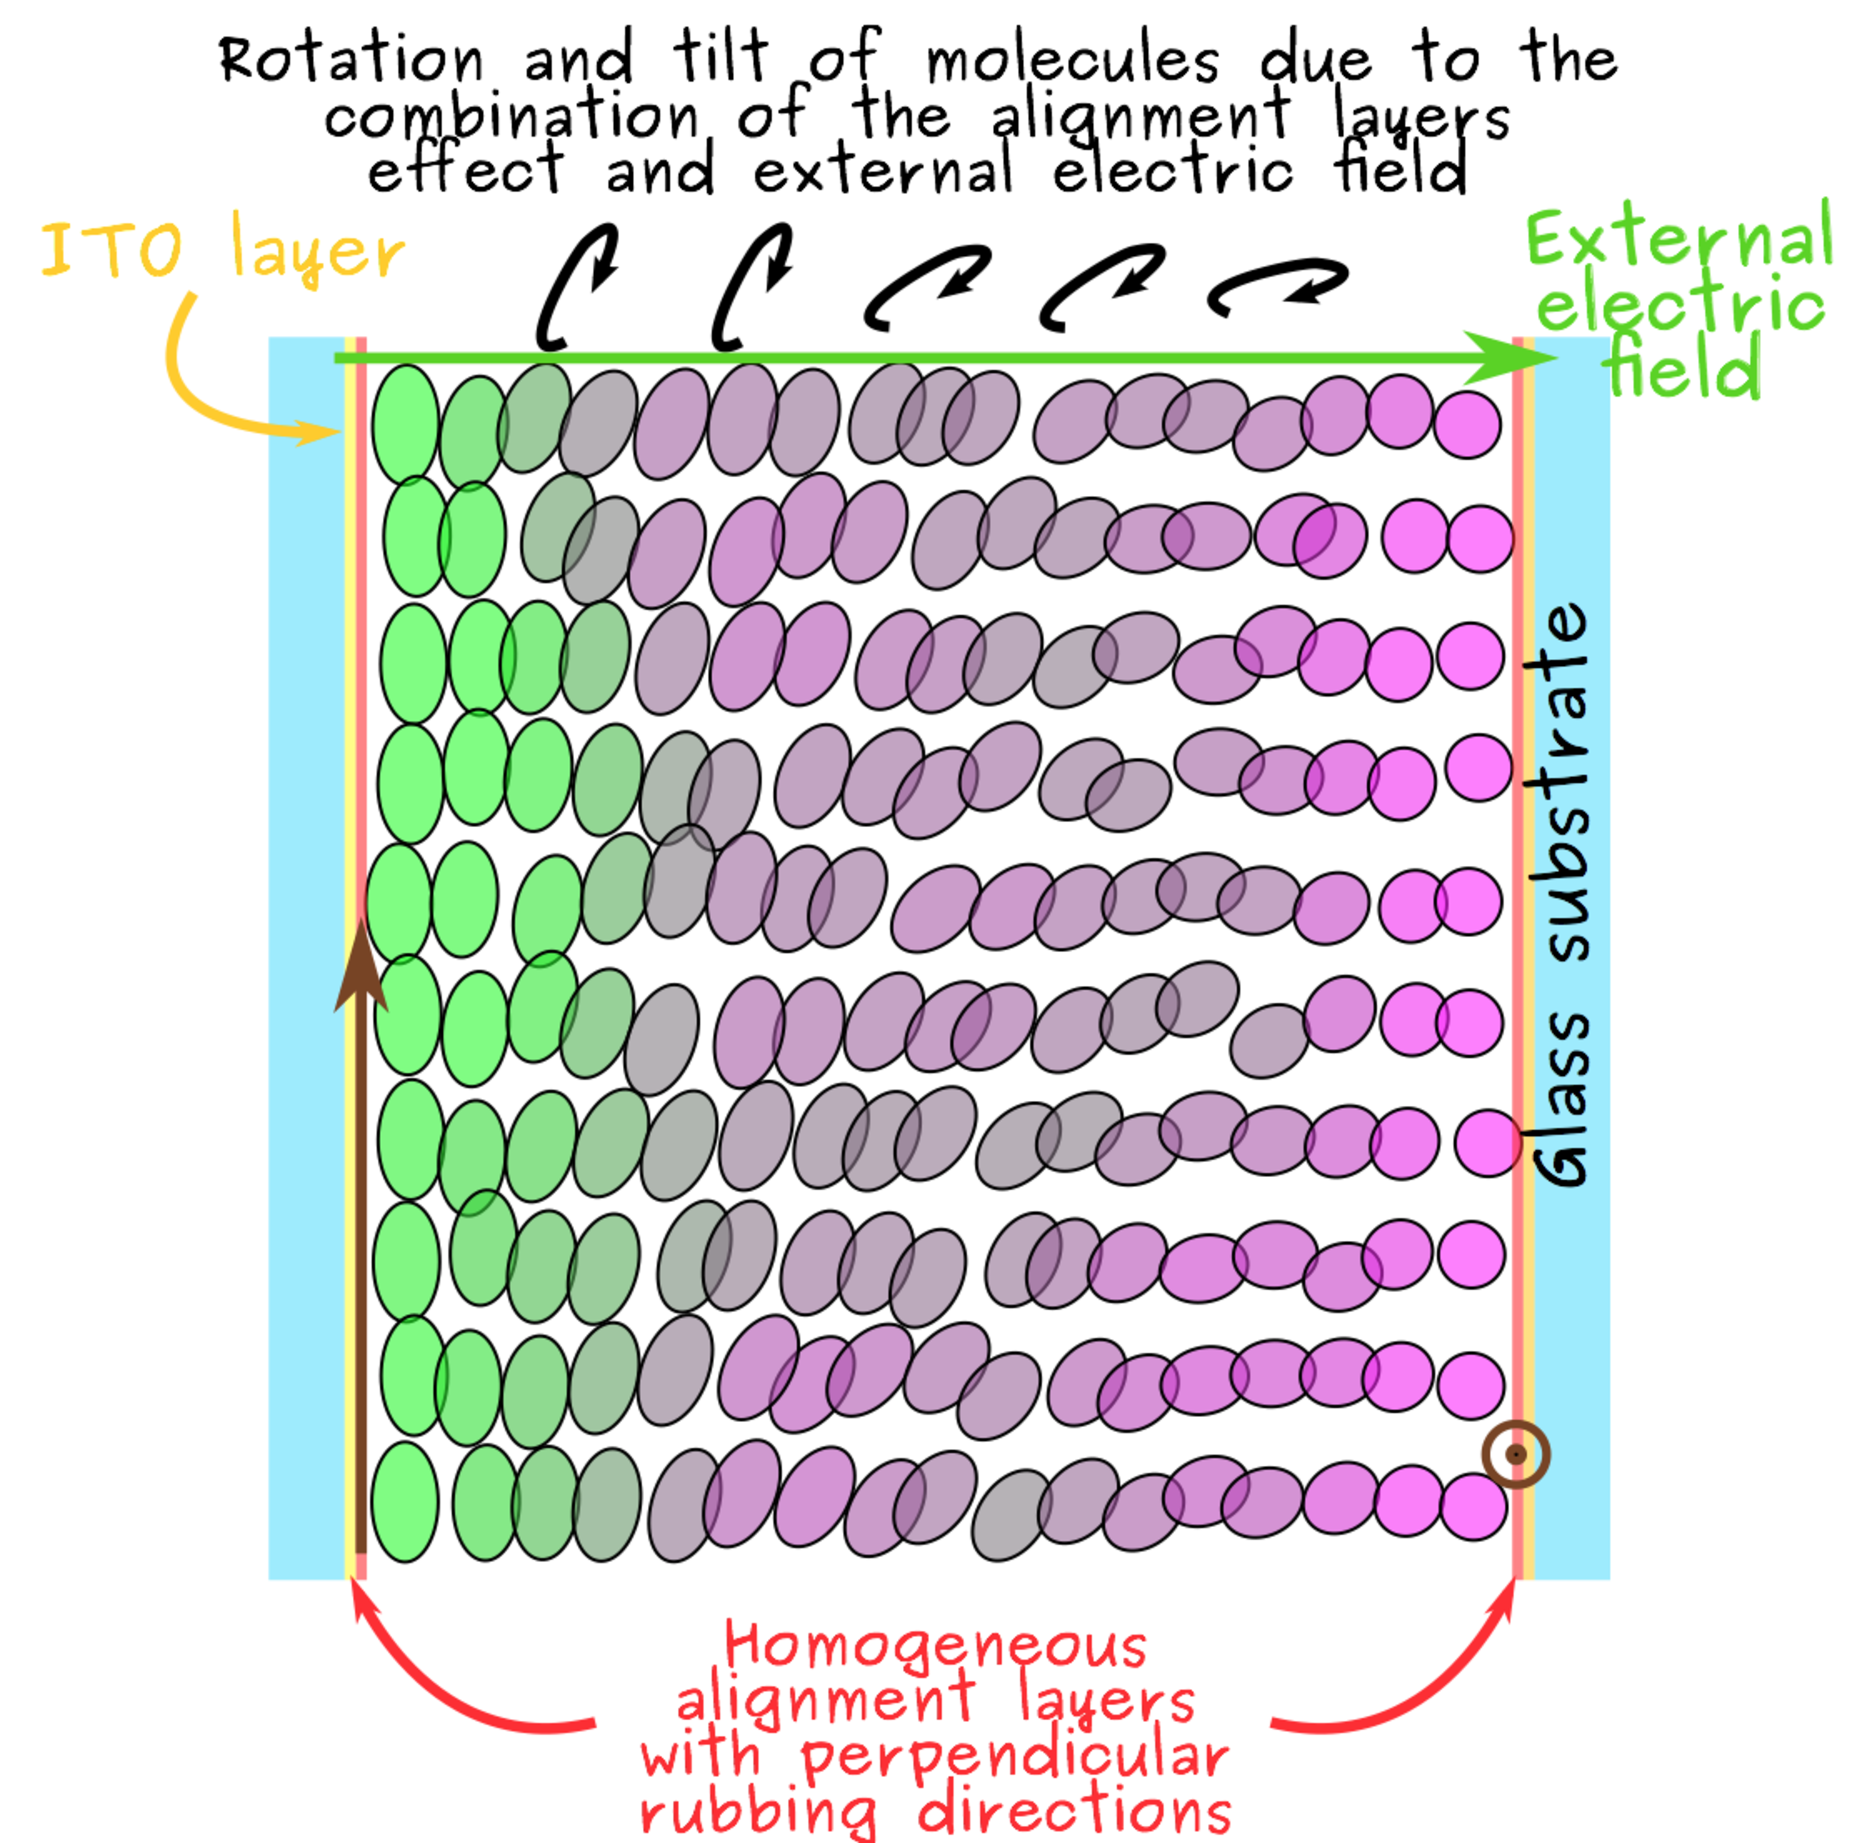
\includegraphics[width=.8\linewidth]{tn-lcd-voltage}
  \caption{Esquema de un TN-LCD dónde se aplica una diferencia de
    potencial entre placas}
  \label{fig:tn-lc-voltage}
\end{subfigure}
\caption[Arquitectura de un TN-LCD]{Arquitectura de un TN-LCD cuando (a) está apagado, y (b) se
  le aplica una diferencia de potencial. Tomado de Nestor Uribe \citepChGen{UribePatarroyo2011}}
  \label{fig:tn-lcd}
\end{figure} 

Generalmente las direcciones de frotado en las superficies de entrada
y salida son ortogonales de tal forma que las moléculas a la salida experimentan
una rotación de 90 grados con respecto a las de la entrada. Ante la
presencia de un campo eléctrico a lo largo del cristal las moléculas
experimentan una inclinación que es proporcional a la diferencia de
potencial entre las placas tal y como se ilustra en la figura
\ref{fig:tn-lc-voltage}. Al ser moléculas alargadas y polares
experimentan un torque que atrae a la parte negativa de la molécula
hacia el electrodo positivo del  dispositivo y viceversa. La
inclinación es proporcional al voltaje aplicado y es de mayor magnitud
en las regiones más alejadas de las paredes del dispositivo. La
configuración Twisted Nematic ha sido seleccionada para muchos
dispositivos electro ópticos comerciales porque afecta 
la polarización de la luz que incide sobre ella. El objetivo de los
autores que han caracterizado moduladores de transmisión ha sido
principalmente el de describir matemáticamente y de forma robusta las
propiedades ópticas de dispositivos que tienen cristales líquidos de esta naturaleza. 

En lo que sigue se presentarán las herramientas matemáticas que son
base para la descripción matemática de campos ópticos polarizados, y
se aplicará para la descripción de un modelo de LC.

\subsection{Polarización de la luz}

En la teoría electromagnética de la luz se representan los campos
ópticos como ondas que se propagan en el espacio vacío. Un haz de luz
se puede representar tanto por su vector de campo eléctrico como
magnético y ambos son perturbaciones de carácter periódico. Si el
medio de propagación es isotrópico, la dirección de la perturbación 
es transversal, es decir ortogonal a la dirección de propagación
($\mathbf{k}\cdot\mathbf{E}$). Para haces planos monocromáticos se
suele usar la siguiente expresión para el campo eléctrico:  

\begin{align}
\mathbf{E} &=\Re\left[\mathbf{A}e^{i\left( \omega t -\mathbf{k}\cdot \mathbf{r}\right)}\right]\label{eq:complex_field},\\
\mathbf{E} &=\mathbf{A}\cos{ \left(\omega t -\mathbf{k}\cdot
    \mathbf{r}\right)},\notag
\end{align}
dónde, $i = \sqrt{-1}$, $\omega$ es la frecuencia temporal, $\mathbf{k}$ es el vector de
onda o frecuencia espacial, y $\mathbf{A}$ determina la amplitud.
Las frecuencias espacial y temporal se relacionan por medio de la
longitud de onda  ($\lambda$) y el índice de refracción del medio ($\mathbf{n}$) con la
siguiente expresión:

$$\mathbf{k} = \mathbf{n} \frac{2\pi}{\lambda}.$$

Dado que son ortogonales, las variaciones del campo se pueden
representar sobre un plano que es 
ortogonal a la dirección de propagación ($z$ en nuestro caso), y ese plano se puede
representar a su vez por dos vectores que son ortogonales entre si
($x$, $y$).
Cuando la variación del campo sucede sobre una dirección preferencial
se dice que la luz es polarizada, y esa dirección se puede descomponer
como una combinación lineal de las variaciones mutuamente independientes
sobre cada uno de los ejes que forman el plano:

\begin{align}
\mathbf{E} &= E_x +E_y, \notag\\
E_x &= A_x\cos{ \left(\omega t -kz+\delta_x\right)} \label{eq:xcomp},\\
E_y &= A_y\cos{ \left(\omega t -kz+\delta_y\right)}\label{eq:ycomp}.
\end{align}

Se ha separado entonces el campo en sus componentes vertical ($y$) y
horizontal ($x$), cada una con su respectiva amplitud ($A_x,A_y$) y
retardo en fase ($\delta_x,\delta_y$). Dado que las amplitudes son
positivas las fases se dan en el rango $-\pi<\delta_{x,y}<\pi$.
La representación en componentes perpendiculares se asemeja a un
sistema acoplado de osciladores armónicos que oscilan a una misma
frecuencia. Si se dibuja la suma vectorial de las componentes $x$, y $y$ como
un vector que va desde el origen hasta el punto ($E_x,E_y$) y luego se
avanza en el tiempo, la trayectoria que describe la punta del vector
será una curva elíptica como la que 
se muestra en la figura \ref{fig:ellipse_clean} . Si en cambio se congela el tiempo y se gráfica
el desplazamiento de la punta del vector en el espacio se obtiene una curva
helicoidal como en la figura \ref{fig:trayectory_clean}. En estos dibujos se ha
escogido representar una elipse por que es el caso más general de polarización. Sin
embargo, la relación entre las amplitudes ($A_y/A_x$) y la
diferencia de fases ($\delta = \delta_y-\delta_x$) entre las componentes del
campo determina si la polarización es lineal ($\delta = 0$), circular
($\delta =\pm \frac{\pi}{2}$) o elíptica, y la orientación del eje
mayor de la elipse con respecto al eje $x$.

\begin{figure}[h!]
\centering
\begin{subfigure}{.45\textwidth}
  \centering
  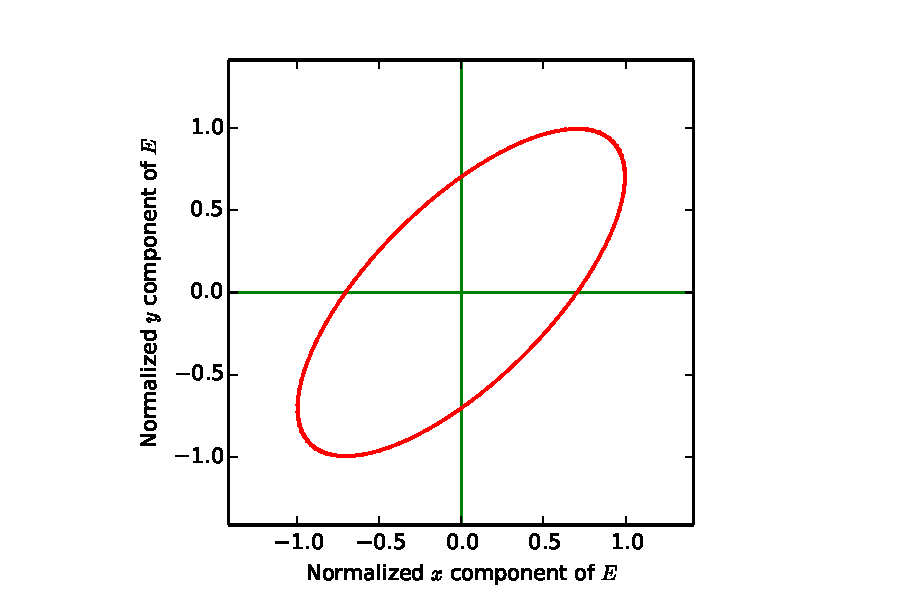
\includegraphics[width=1\linewidth]{ellipse_clean}
  %\caption{Elipse arbitraria que resulta cuando se observa la
   % variación temporal de un campo sobre el plano.}
  \caption{}
\label{fig:ellipse_clean}
\end{subfigure}\qquad
\begin{subfigure}{.45\textwidth}
  \centering
  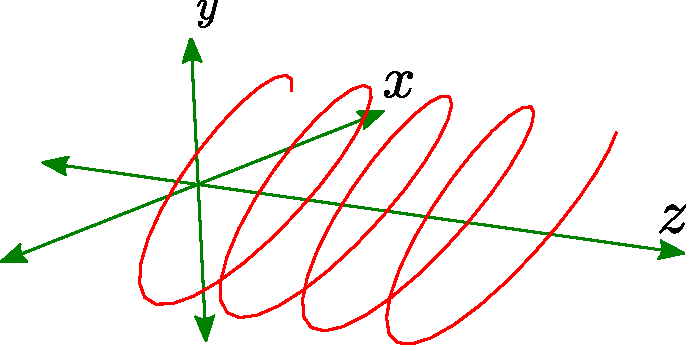
\includegraphics[width=.8\linewidth]{trayectory_clean}
 % \caption{Trayectoria helicodidal de la variación espacial de un
  %  campo óptico a lo largo de $z$.}
  \caption{}
  \label{fig:trayectory_clean}
\end{subfigure}
\caption[Distintas representaciones del campo eléctrico para ilustrar
la polarización]{Representaciones de la posición de un vector de campo
  eléctrico con polarización elíptica cuando (a) se analiza en un
  punto en el espacio, y (b) se  congela el tiempo.} 
\label{fig:general_field}
\end{figure} 

Desde el punto de vista matemático, la figura
\ref{fig:ellipse_clean} se describe por medio de la ecuación
\ref{eq:ellipse} que es la ecuación de una cónica y se puede obtener
a partir de las expresiones (\ref{eq:xcomp}) y (\ref{eq:ycomp}) como se
muestra a continuación. Si $\delta = \delta_y-\delta_x$ y $z=0$,
entonces el campo se puede escribir como

\begin{align*}
E_x &= A_x\cos{ \left(\omega t \right)},\\
E_y &= A_y\cos{ \left(\omega t -\delta\right)}.
\end{align*}
Y se puede despejar los términos correspondientes al $\sin$ y $\cos$
 \begin{align*}
\cos{\omega t} &=\frac{E_x}{A_x},\\
\sin^2{\omega t} &= 1-\left(\frac{E_x}{A_x}\right)^2,\\
\sin{\omega t} &= \sqrt{1-\left(\frac{E_x}{A_x}\right)^2}.
\end{align*}
Por otra parte se tiene
\begin{equation}
  \label{eq:Ey-2}
E_y = A_y\left( \cos{\omega t}\cos{\delta}+\sin{\omega
    t}\sin{\delta}\right).  
\end{equation}
Reemplazando $\sin{\omega t} $ y $\cos{\omega t} $ en la expresión
(\ref{eq:Ey-2}) obtenemos
\begin{align}
E_y &= \frac{A_yE_x}{A_x}\cos{\delta} +
A_y\sqrt{1-\frac{E_x}{A_x}}\sin{\delta},\notag\\
\frac{E_y}{A_y} - \frac{E_x}{A_x}\cos{\delta}  &= 
\sqrt{1-\left(\frac{E_x}{A_x}\right)^2}\sin{\delta}.\label{eq:ellipse_nos}
\end{align}
Elevando al cuadrado la igualdad (\ref{eq:ellipse_nos}) y organizando
términos, obtenemos la ecuación general de una elipse inscrita en un
rectángulo con lados $2A_x$, $2A_y$: 
\begin{equation}
\left(\frac{E_x}{A_x}\right)^2+\left(\frac{E_y}{A_y}\right)^2-2\frac{\cos{\delta}}{A_xA_y}E_xE_y
= \sin^2{\delta}.
\label{eq:ellipse}
\end{equation}
Se puede ahora plantear una rotación de un ángulo $\phi$ con respecto
al eje horizontal ($x$) sobre el sistema de coordenadas  como se
muestra en la figura \ref{fig:ellipse} para que
el eje mayor de la elipse quede alineado con el eje
\textit{horizontal} del nuevo sistema. 
\begin{figure}[h!]
\centering
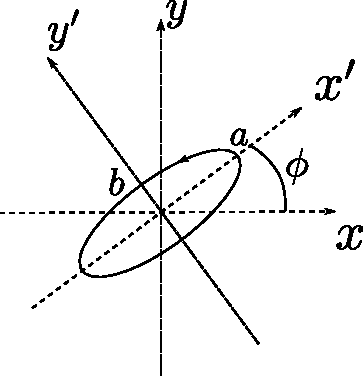
\includegraphics[scale = 1]{ellipse}
\caption[Rotación del sistema de coordenadas de la elipse de polarización]{Rotación del sistema de coordenadas un ángulo $\phi$.}
\label{fig:ellipse}
\end{figure}
Haciendo esto, se lleva la
ecuación (\ref{eq:ellipse}) a la forma más conocida de la ecuación
(\ref{eq:new_ellipse})
\begin{equation}
\left(\frac{E_{x'}}{a}\right)^2+\left(\frac{E_{y'}}{b}\right)^2 = 1,
\label{eq:new_ellipse}
\end{equation}
dónde $a$ y $b$ son los semi ejes mayor y menor, y $E_{x'}$, $E_{y'}$
son las componentes del campo eléctrico en las direcciones $x'$,
$y'$. Los semiejes de la elipse están dados por las siguientes expresiones:
\begin{align*}
a^2 = A_x\cos^2{\phi}+A_y^2\sin^2{\phi} +2A_xA_y \cos{\delta}\cos{\phi}\sin{\phi},\\
b^2 = A_x\sin^2{\phi}+A_y^2\cos^2{\phi} -2A_xA_y \cos{\delta}\cos{\phi}\sin{\phi}.
\end{align*}

La elipticidad se define como la razón entre el eje menor y el eje
mayor de la elipse $e=\pm\frac{b}{a}$ de tal forma que si el semi eje
menor es cero, la elipse se vuelve una linea y por tanto se dice que
la polarización es lineal en la dirección de $a$. Si por el contrario
los dos semi ejes tienen  la misma longitud, la ecuación de la elipse
se vuelve la de un círculo, y se dice que la polarización es
circular como en la figura \ref{fig:circular_polarizations}a. 
El signo de la elipticidad determina el sentido
de giro de la hélice, si el signo es positivo la elipse es circular
izquierda como en la figura \ref{fig:circular_polarizations}b y es circular derecha
cuando el signo es negativo \ref{fig:circular_polarizations}c. Cabe
anotar que el sentido de giro de la polarización es una convención
que varía según el autor, algunos interpretan el sentido de giro como
si se congelara el tiempo y se siguiera la punta del vector
$\mathbf{E}$ desde el cero en adelante. Sin embargo otros autores
interpretan el sentido de giro como si en un punto fijo vieran girar
el vector $\mathbf{E}$ que les llega en la medida que pasa el tiempo. 

\begin{figure}[h!]
\centering
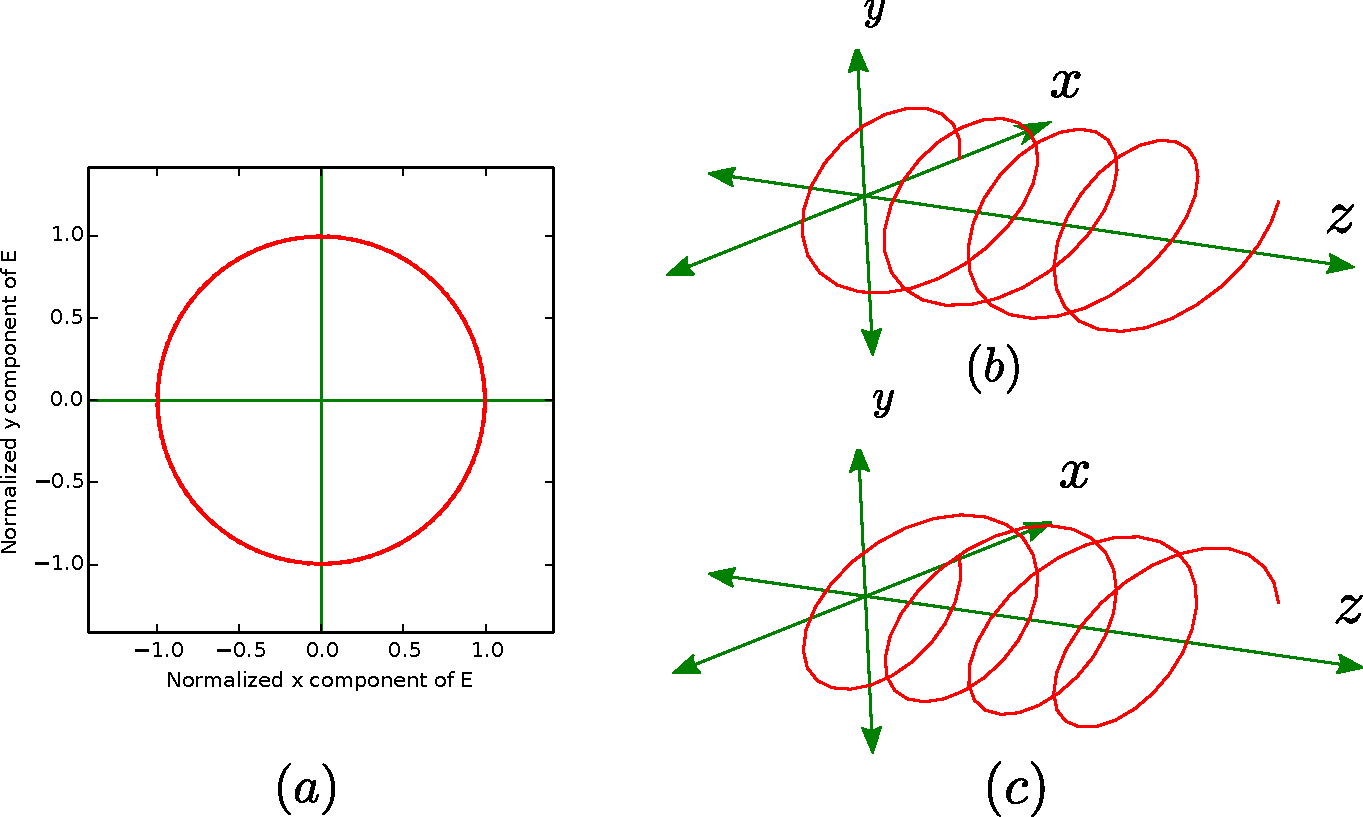
\includegraphics[scale=.5]{circular_polarizations}
\caption[Estados de polarización circular]{(a) Esquema de un estado de polarización circular en donde los semiejes
  de la elipse son iguales. La polarización circular izquierda (b) se da
cuando $e=\frac{b}{a}$ y la derecha (c) cuando  $e=-\frac{b}{a}$.}
\label{fig:circular_polarizations}
\end{figure}

Una ellipse de polarización arbitraria se puede expresar entonces conociendo su
elipticidad y su ángulo de inclinación con respecto al eje
horizontal. Estas dos características se pueden parametrizar como dos
ángulos que se dan en
términos de las amplitudes máximas del campo $A_x$, $A_y$
y el retardo entre componentes $\delta$. Por una parte, el ángulo de
inclinación se encuentra interpretando la ecuación (\ref{eq:ellipse}) en
su forma bilineal de la forma

\begin{equation}
\begin{pmatrix}
E_x & E_y
\end{pmatrix}
\begin{pmatrix}
\frac{1}{A_x^2} & -\frac{\cos{\delta}}{A_xA_y}\\
 -\frac{\cos{\delta}}{A_xA_y} & \frac{1}{A_y^2} 
\end{pmatrix}
\begin{pmatrix}
E_x \\ E_y
\end{pmatrix}
=\sin^2{\delta},
\end{equation}

sacando factor común $\frac{1}{A_x^2} $ se obtiene

\begin{equation}
\begin{pmatrix}
E_x & E_y
\end{pmatrix}
\begin{pmatrix}
1 & -\frac{A_x\cos{\delta}}{A_y}\\
 -\frac{A_x\cos{\delta}}{A_y} & \frac{A_x/2}{A_y^2} 
\end{pmatrix}
\begin{pmatrix}
E_x \\ E_y
\end{pmatrix}
=A_x/2\sin^2{\delta},
\end{equation}
o en forma compacta
\begin{equation}
\begin{pmatrix}
E_x & E_y
\end{pmatrix}
\begin{pmatrix}
1 & a\\
 a & b 
\end{pmatrix}
\begin{pmatrix}
E_x \\ E_y
\end{pmatrix}
=c.
\end{equation}
%http://mpalffy.lci.kent.edu/Optics/Chapters/Ch7_Polarized%20Light.pdf

Una \href{http://es.wikipedia.org/wiki/Cu\%C3\%A1drica}{cuádrica o
  superficie cuádrica} es una  hipersuperficie D-dimensional
representada por una ecuación de segundo grado con 
coordenadas espaciales. Si estas coordenadas son $\{x_1,
x_2, ... x_D\}$, entonces la cuádrica típica en ese espacio se define
mediante la ecuación algebraica: 
\[ \sum_{i,j=1}^D Q_{i,j} x_i x_j + \sum_{i=1}^D P_i x_i + R = 0. \]
El caso particular en el cual solo hay dos dimensiones y los valores
$P_i$ son todos 0, es el de una elipse. En nuestro caso, tenemos en
notación matricial:
\[ \mathbf{E}^TQ\mathbf{E} + R= 0, \]
con
\[
Q=
\begin{pmatrix}
1 & a\\
 a & b 
\end{pmatrix}.
 \]
y $R=-c = -A_x/2\sin^2{\delta}$. Ahora, los autovalores de una elipse
representada por su forma matricial están asociados con la
dirección de sus ejes principales, y apuntan en la dirección de los
puntos máximos \citepChGen{Palffy1998}. Como nuestra incógnita es el ángulo
que determina la dirección de los puntos máximos, podemos escribir la
siguiente ecuación de autovalores para despejar $\phi$\footnote{
\url{http://en.wikipedia.org/wiki/Quadratic_form}}
\[\begin{pmatrix}
1 & a\\
 a & b 
\end{pmatrix} 
\begin{pmatrix}
\cos{\phi}\\
 \sin{\phi} 
\end{pmatrix} =
\lambda \begin{pmatrix}
\cos{\phi}\\
 \sin{\phi} 
\end{pmatrix} ,
\]
desarrollando, se obtienen las siguientes dos ecuaciones:
\begin{align*}
\cos{\phi} +a\sin{\phi} &= \lambda\cos{\phi},\\
a\cos{\phi} +b\sin{\phi} &= \lambda\sin{\phi}.
\end{align*}
Despejando $\lambda$ e igualando las ecuaciones se llega a una
expresión dependiente de un ángulo doble:
\[1+a\tan{\phi} = \frac{a}{\tan{\phi}}+b,\]
\[b-1= a\tan{\phi} -\frac{a}{\tan{\phi}},\]
\[ b-1=a\left(\frac{\tan^2{\phi} -1}{\tan{\phi}}\right),\]
\[\tan{2\phi} =\frac{2a}{b-1}.\]
Finalmente, reemplazando $a$, y $b$ se tiene el ángulo de inclinación
de la elipse:
\begin{equation*}
\phi = \frac{1}{2}\tan^{-1}{\left(\frac{2A_xA_y}{A_x^2-A_y^2}\cos{\delta}\right)}.
\end{equation*}
Siguiendo un esquema similar, aunque más tedioso se encuentra el
ángulo de elipticidad ($\theta = \tan^{-1}{e}$) en términos de la
función seno como:
\begin{equation*}
\theta = \frac{1}{2}\sin^{-1}{\left(\frac{2A_xA_y}{A_x^2+A_y^2}\sin{\delta}\right)}.
\end{equation*}
A la hora de despejar $\phi$ y $\theta$ reemplazando valores en la
primera ecuación usando un computador se aconseja reemplazar la función
$\tan^{-1}$ por la función atan2, que es popular en paquetes de
cálculos numéricos (como numpy) o lenguajes de programación como
Matlab, porque permite evitar las singularidades que ocurren cuando el argumento de la
función tangente inversa es $\pi/2$.

\subsection{El formalismo de Jones}

Se conoce como formalismo de Jones al uso de una representación
vectorial para describir campos ópticos coherentes y monocromáticos cuando es
importante la naturaleza vectorial de la luz y la polarización.  
En el esquema de Jones los campos ópticos con dos componentes ortogonales se
representan como un vector con elementos complejos conocido como
vector de Jones. Las dos componentes complejas del campo en la ecuación
(\ref{eq:complex_field}) se representan como elementos de un vector
columna conocido como vector de Jones:
 
\begin{equation}
\mathbf{J} =\begin{pmatrix} A_xe^{i\delta_x}\\A_ye^{i\delta_y}\end{pmatrix}.
\label{eq:jones_vector}
\end{equation}
Siendo un vector complejo, $\mathbf{J}$ no es una cantidad observable
en el espacio físico. Para obtener obtener por ejemplo, la
componentente  $x$ del campo eléctrico se hace la operación $E_x(t) = \Re
\left[J_xe^{i\omega t}\right]$.
Para el estudio de la polarización conviene representar el vector de
Jones en su forma normalizada, es decir tal que cumpla la
condición $$\mathbf{J}^{\dagger}\mathbf{J}=1,$$
dónde el símbolo $\dagger$ representa la transpuesta conjugada.
La normalización se logra parametrizando las amplitudes con el ángulo
del vector que forman: $$\tan{\psi}=\frac{\sin{\psi}}{\cos{\psi}}=\frac{A_y}{A_x},$$
de esta forma $A_y=\sin{\psi}$ y $A_x = \cos{\psi}$. Adicionalmente,
la fase de las componentes se acostumbra a escribir en su forma
relativa y con respecto a la componente $y$ como se muestra en la
expresión (\ref{eq:normalized_jones_vector}).

\begin{equation}
\mathbf{J(\psi,\delta)} =\begin{pmatrix} \cos{\psi}\\\sin{\psi}e^{i\delta}\end{pmatrix}.
\label{eq:normalized_jones_vector}
\end{equation}

\subsubsection{Algunos estados de polarización importantes}
Como se dijo antes, las polarizaciones lineales se obtienen cuando las
componentes están en fase, es decir que $\delta =
\delta_y-\delta_x=0$. Sin embargo, la condición también se cumple cuando las
diferencias de fase entre las componentes son múltiplos de $\pi$. 
Por otra parte, las polarizaciónes lineales ($\delta = n\pi$ ) horizontal y vertical se dan cuando $\psi
= n\pi$ y $\psi = \frac{\pi}{2}(2n+1)$ respectivamente:
\begin{align*}
\mathbf{H} &=\begin{pmatrix}1\\0\end{pmatrix},& \mathbf{V} &=\begin{pmatrix}0\\1\end{pmatrix}.
\end{align*}
Y la polarización lineal a $45^{\circ}$ se da cuando las componentes $x$
y $y$ tienen la misma magnitud y dirección, es decir cuando
$\psi=\frac{\pi}{4}(4n+1)$. La polarización a  $-45^{\circ}$ se da cuando
$\psi=\frac{\pi}{4}(4n-1)$.
\begin{align*}
\mathbf{45^{\circ}}
&=\begin{pmatrix}\cos{\pi/4}\\\sin{\pi/4}\end{pmatrix}=\frac{1}{\sqrt{2}}
\begin{pmatrix}1\\1\end{pmatrix},&
\mathbf{-45^{\circ}} 
&=\begin{pmatrix}\cos{-\pi/4}\\\sin{-\pi/4}\end{pmatrix}=\frac{1}{\sqrt{2}}\begin{pmatrix}1\\-1\end{pmatrix}. 
\end{align*} 
Las polarizaciones circular izquierda y circular derecha son tales que
ambas componentes tienen la misma magnitud como en la de $45^{\circ}$,
pero el retardo en fase es de $\delta = \frac{\pi}{2}$:
\begin{align*}
\mathbf{CD}
&=\begin{pmatrix}\cos{\pi/4}\\\sin{\pi/4}e^{i\frac{\pi}{2}}\end{pmatrix}=\frac{1}{\sqrt{2}}
\begin{pmatrix}1\\i\end{pmatrix},&
\mathbf{CI} 
&=\begin{pmatrix}\cos{-\pi/4}\\\sin{-\pi/4}e^{i\frac{\pi}{2}}\end{pmatrix}=\frac{1}{\sqrt{2}}\begin{pmatrix}1\\-i\end{pmatrix}. 
\end{align*} 
Una característica interesante de los estados lineales y circulares es
que se pueden dar unos como combinación lineal de los otros:
\begin{align*}
\mathbf{CD} &= \frac{1}{\sqrt{2}}\left( \mathbf{H} -
  i\mathbf{V}\right),\\
\mathbf{CI} &= \frac{1}{\sqrt{2}}\left( \mathbf{H} +
  i\mathbf{V}\right),\\
\mathbf{H} &= \frac{1}{\sqrt{2}}\left( \mathbf{CD} +
  \mathbf{CI}\right),\\
\mathbf{V} &= \frac{i}{\sqrt{2}}\left( \mathbf{CD} -
  \mathbf{CI}\right).
\end{align*}
Los vectores de las tres parejas de estados que hemos visto hasta
ahora son bases
ortonormales. Esto quiere decir que fuera de estar normalizados,
%son linealmente independientes entre sí, 
si calculamos el producto escalar elementos de una misma pareja obtenemos un
valor de 0,
% \begin{equation*}
% \begin{pmatrix}1&0\end{pmatrix}\begin{pmatrix}0\\1\end{pmatrix}=
% \left(\frac{1}{\sqrt{2}}\begin{pmatrix}1&1\end{pmatrix}\right)\left(\frac{1}{\sqrt{2}}\begin{pmatrix}1\\-1\end{pmatrix}\right)  = \left(\frac{1}{\sqrt{2}}
% \begin{pmatrix}1&i\end{pmatrix}\right)\left(\frac{1}{\sqrt{2}}\begin{pmatrix}1\\-i\end{pmatrix}\right)
% = 0.
% \end{equation*}
\begin{equation*}
\mathbf{H^{\dagger}V} = \mathbf{45^{\circ\dagger}45^{\circ}} =
\mathbf{CD^{\dagger}CI = 0.}   
\end{equation*}
Fuera de eso, estos estados se han mencionado porque sirven como base para el espacio
de posibles estados de polarización y serán usados en la sección
\ref{sec:ChGV_med_mod_amp} para producir 6 curvas de modulación de
amplitud que alimentan un modelo inspirado en el de \citetChGen{Ma2010}  capaz de predecir la modulación para
cualquier otro estado. 

\subsubsection{Elementos ópticos como operadores en la representación
  de Jones}

Así como en el álgebra lineal se usan matrices para transformar
vectores, en el formalismo de Jones existen operadores que se
representan como matrices 2x2 y que tienen la cualidad de
transformar los campos. Estos operadores se conocen como matrices de
Jones y deben cumplir algunas
propiedades generales \citepChGen{Yariv2002} que se listan a continuación:

\begin{enumerate}
\item La dirección de propagación de un campo determina las
  componentes de la matriz que representa al elemento polarizador. Si
  la incidencia es desde la izquierda $(z=0)$ definimos la matriz $M$ como aquella
  que transforma el vector de entrada en el de salida

  \begin{equation}
    \begin{pmatrix}
      V_x^{out}\\V_y^{out}
    \end{pmatrix}
    =
    \begin{pmatrix}
      M_{11}&M_{12}\\M_{21} & M_{22}
    \end{pmatrix}
    \begin{pmatrix}
      V_x^{in}\\V_y^{in}
    \end{pmatrix},
    \label{eq:right_propagation}
  \end{equation}
si el vector de entrada ingresa desde la derecha entonces
definiremos una matriz distinta $N$ para representar la transformación:
  \begin{equation*}
    \begin{pmatrix}
      V_x^{out}\\V_y^{out}
    \end{pmatrix}
    =
    \begin{pmatrix}
      N_{11}&N_{12}\\N_{21} & N_{22}
    \end{pmatrix}
    \begin{pmatrix}
      V_x^{in}\\V_y^{in}
    \end{pmatrix}.
  \end{equation*}

Para que se cumpla el principio de simetría temporal, se debe cumplir
que $NM=1$. Si se rebobina la propagación en la expresión
(\ref{eq:right_propagation}) el haz de salida 
debería seguir el mismo camino que recorrió a la entrada, y ser
afectado por la matriz $N$ de tal forma que vuelva a la forma que
tenía en un principio 

 \begin{align*}
    \begin{pmatrix}
      V_x^{in}\\V_y^{in}
    \end{pmatrix}
    &=
    \begin{pmatrix}
      N_{11}&N_{12}\\N_{21} & N_{22}
    \end{pmatrix}
    \begin{pmatrix}
      V_x^{out}\\V_y^{out}
    \end{pmatrix},\\
    &=
    \begin{pmatrix}
      N_{11}&N_{12}\\N_{21} & N_{22}
    \end{pmatrix}
    \begin{pmatrix}
      M_{11}&M_{12}\\M_{21} & M_{22}
    \end{pmatrix}
    \begin{pmatrix}
      V_x^{in}\\V_y^{in}
    \end{pmatrix}.\\
  \end{align*}
  Conociendo que las matrices están asociadas a un mismo elemento se
  debe cumplir que $N$ sea la transpuesta de $M$
  \begin{align*}
    N_{11}&=M_{11},&    N_{12}&=M_{21},&     N_{21}&=M_{12}, &     N_{22}&=M_{22}.
  \end{align*}
Esta relación es importante para analizar sistemas en los cuales la
luz debe pasar dos veces por el LC en sentidos opuestos, caso especial
es el de los SLM's de reflexión en los cuales hay una
superficie especular de un lado.

\item Tanto la matriz $M$ como la $N$ son operadores unitarios:
  \begin{align*}
    M^{\dagger} M &= 1,& N^{\dagger}N &=1.
  \end{align*}
Dónde el símbolo $\dagger$ indica que se saca el conjugado hermítico
de $M$:
\begin{equation*}
M^{-1}=M^{\dagger}=
  \begin{pmatrix}
      M_{11}^*&M_{21}^*\\M_{12}^* & M_{22}^*
    \end{pmatrix}.
\end{equation*}
\item Las matrices de Jones son unimodulares es decir
$$det(M) = det(M^{\dagger})  = M_{11}M_{22}-M_{12}M_{21} = 1.$$ 
Si asumimos que $M^{-1}$ es
\begin{equation*}
  M=
  \begin{pmatrix}
    M_{22}&-M_{12}\\-M_{21}&M_{11}
  \end{pmatrix},
\end{equation*}
se ve que cumple con la relación $M^{-1}M = 1$:
\begin{align*}
    \begin{pmatrix}
    M_{22}&-M_{12}\\-M_{21}&M_{11}
  \end{pmatrix}
\begin{pmatrix}
      M_{11}&M_{12}\\M_{21} & M_{22}
    \end{pmatrix}
&=
    \begin{pmatrix}
 M_{22}M_{11}-M_{12}M_{21}     & M_{22}M_{12}-M_{12}M_{22}\\
-M_{11}M_{21}+M_{11}M_{21}    & -M_{12}M_{21} + M_{11}M_{22} 
    \end{pmatrix},\\
&=
\begin{pmatrix}
  1 &0\\0&1
\end{pmatrix}.
\end{align*}
Con esto, se puede simplificar la forma de una matriz de Jones a
partir de las siguientes relaciones:
\begin{align*}
  M_{21} &= - M_{12}^*, & M_{22} = M_{11}^*,
\end{align*}
obteniendo una forma de la matriz que depende de sólo dos números
complejos:
\begin{align}
  M&=
  \begin{pmatrix}
    A & B \\-B^* & A^*
  \end{pmatrix}\\
&=
  \begin{pmatrix}
    x+iy & z+iw \\-z+iw & x-iy
  \end{pmatrix}
\label{eq:general_jones_matrix}
\end{align}

Tener la matriz en esta forma facilita encontrar los parámetros de elementos
ópticos desconocidos como un SLM porque reduce el número de incógnitas.

\end{enumerate}

Los operadores que se verán a
continuación hacen referencia a dos tipos de elementos ópticos que se
utilizan en el laboratorio para modificar los estados de polarización
de una onda, estos son, polarizadores y retardadores. Los polarizadores
son elementos que afectan únicamente la amplitud y los
retardadores introducen retardos de la fase entre las componentes del campo.
Por una parte, los polarizadores horizontales son elementos que sólo
dejan pasar la componente $x$ del campo, y se representan con la
matriz de la expresión (\ref{eq:Px_matrix}).
\begin{equation}
P_x = \begin{pmatrix}1 &0\\0&0\end{pmatrix}.
\label{eq:Px_matrix}
\end{equation}
Si llega cualquier campo al polarizador horizontal este dejará pasar
sólo la componente $x$ tal y
como se muestra en la figura \ref{fig:linear_polarizer}. 
\begin{figure}[h!]
\centering
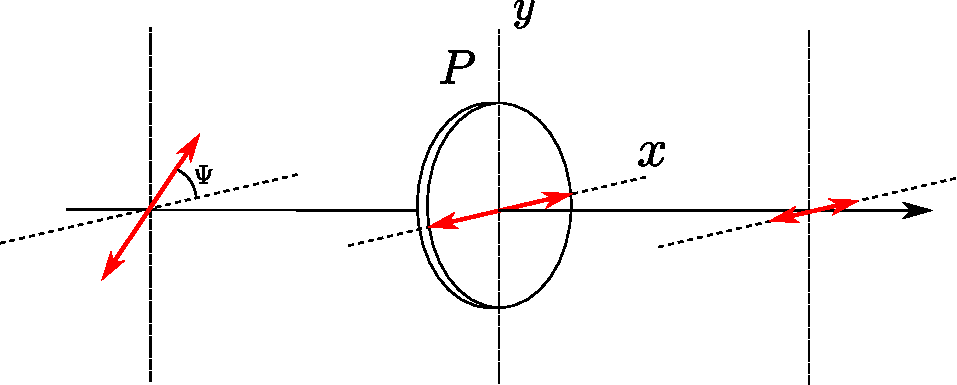
\includegraphics[scale = .7]{linear_polarizer}
\caption{Propagación de un estado de polarización lineal a través de
  un polarizador horizontal.}
\label{fig:linear_polarizer}
\end{figure}
La  operación vectorial correspondiente a este fenómeno se da como la
multiplicación entre la matriz del polarizador y el vector de Jones
que representa al campo, en este caso un campo con polarización lineal
a $45^{\circ}$
\begin{equation*}
\frac{1}{\sqrt{2}}
\begin{pmatrix}
1\\0
\end{pmatrix}
=
\begin{pmatrix}
1 &0\\0&0
\end{pmatrix}
\frac{1}{\sqrt{2}}
\begin{pmatrix}
1 \\1
\end{pmatrix}.
\end{equation*}
Los polarizadores que no están orientados con el eje $x$ se pueden
obtener a partir de la matriz de $P_x$ por medio de la siguiente
operación de rotación, 
\begin{align*}
P_{\theta}&=R^T(\theta)P_xR(\theta)\\
P_{\theta}
&=
\begin{pmatrix}
  \cos{\theta} &-\sin{\theta}\\\sin{\theta}&\cos{\theta}
\end{pmatrix},
\begin{pmatrix}
1 & 0 \\0& 0
\end{pmatrix}
\begin{pmatrix}
  \cos{\theta} &\sin{\theta}\\-\sin{\theta}&\cos{\theta}
\end{pmatrix}.
\end{align*}
En adelante se seguirá usando este método para representar la matriz de cualquier
elemento óptico rotado.
Reemplazando $\theta = \frac{\pi}{2}$ y $\theta = \frac{\pi}{4}$
obtenemos las matrices $P_V$ y $P_{45^{\circ}}$ correspondientes al
polarizador horizontal y al que está inclinado $45^{\circ}$:
\begin{align*}
P_{V}
&=
\begin{pmatrix}
  \cos{\frac{\pi}{2}} &-\sin{\frac{\pi}{2}}\\\sin{\frac{\pi}{2}}&\cos{\frac{\pi}{2}}
\end{pmatrix}
\begin{pmatrix}
1 & 0 \\0& 0
\end{pmatrix}
\begin{pmatrix}
  \cos{\frac{\pi}{2}} &\sin{\frac{\pi}{2}}\\-\sin{\frac{\pi}{2}}&\cos{\frac{\pi}{2}}
\end{pmatrix},\\
&=
\begin{pmatrix}
  0&-1\\1&0
\end{pmatrix}
\begin{pmatrix}
1 & 0 \\0& 0
\end{pmatrix}
\begin{pmatrix}
0 &1\\-1&0
\end{pmatrix},\\
&=
\begin{pmatrix}
0 &0\\0&1
\end{pmatrix}.\\
\end{align*}
\begin{align*}
P_{45^{\circ}}
&=
\begin{pmatrix}
  \cos{\frac{\pi}{4}} &-\sin{\frac{\pi}{4}}\\\sin{\frac{\pi}{4}}&\cos{\frac{\pi}{4}}
\end{pmatrix}
\begin{pmatrix}
1 & 0 \\0& 0
\end{pmatrix}
\begin{pmatrix}
  \cos{\frac{\pi}{4}} &\sin{\frac{\pi}{4}}\\-\sin{\frac{\pi}{4}}&\cos{\frac{\pi}{4}}
\end{pmatrix},\\
&=
\frac{1}{\sqrt{2}}
\begin{pmatrix}
  1&-1\\1&1
\end{pmatrix}
\begin{pmatrix}
1 & 0 \\0& 0
\end{pmatrix}
\frac{1}{\sqrt{2}}
\begin{pmatrix}
1 &1\\-1&1
\end{pmatrix},\\
&=
\frac{1}{2}
\begin{pmatrix}
1 &1\\1&1
\end{pmatrix}.\\
\end{align*}
Por otra parte, los retardadores ópticos modifican tanto la amplitud
como la fase de las componentes del campo y sus elementos son
complejos. La matriz general para un retardador óptico con desfase
$\beta $ y orientación del eje rápido con el eje
$x$ es:
\begin{equation}
WP = 
\begin{pmatrix}
e^{i\beta/2} & 0 \\0&e^{-i\beta/2}  
\end{pmatrix}
\label{eq:retarder}
\end{equation}
Los retardadores ópticos se construyen a partir de materiales
birrefringentes donde el retardo de fase $\beta$ de una componente con respecto a otra es
proporcional a la diferencia de índices de refracción, y a la
profundidad $d$ del medio birrefringente,
$$\beta= \frac{\pi}{2}d\left(n_e-n_o\right).$$ 
Dónde el índice de refracción extraordinario corresponde al eje rápido
del medio, y el extraordinario al eje lento. Si multiplicamos la
ecuación (\ref{eq:retarder}) por $e^{-i\beta/2} $ 
obtenemos la forma no normalizada que es muy común en los libros de
texto porque en ella se hace evidente que la componente $E_y$ del campo sufre un
retardo en fase de $\beta$ con respecto a $E_x$: 
\begin{equation*}
WP = 
\begin{pmatrix}
1& 0 \\0&e^{-i\beta}  
\end{pmatrix}.
\label{eq:retarder_2}
\end{equation*}
Los retardadores más usados en el laboratorio son aquellos que
introducen retardos de cuarto de onda:
\begin{align*}
QWP &= \begin{pmatrix} e^{i\frac{\pi}{4}}  &0\\0&e^{-i\frac{\pi}{4}}\end{pmatrix},\\
&=  \begin{pmatrix} 1 &0\\0&e^{-i\frac{\pi}{2}}\end{pmatrix},\\
&=  \begin{pmatrix} 1 &0\\0&-i\end{pmatrix},
\end{align*}
y retardos de
media onda:
\begin{align*}
HWP &= \begin{pmatrix} e^{i\frac{\pi}{2}}  &0\\0&e^{-i\frac{\pi}{2}}\end{pmatrix},\\
&=  \begin{pmatrix} 1 &0\\0&e^{-i\frac{\pi}{2}}\end{pmatrix},\\
&=  \begin{pmatrix} 1 &0\\0&-1\end{pmatrix},\\
\end{align*}
Los de cuarto de onda permiten obtener polarizaciones
circulares o elípticas a partir de polarizaciones lineales. La figura
\ref{fig:qwp_retarder} muestra cómo conseguir un campo con
polarización circular derecha a partir de polarización lineal y un 
retardador $QWP$.
\begin{figure}[h!]
\centering
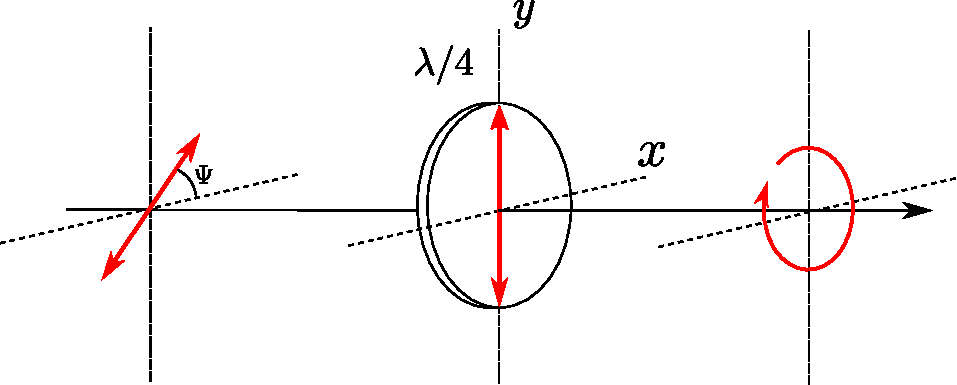
\includegraphics[scale=.7]{qwp_retarder}
\caption[Generación de estados de polarización circulares]{Propagación de un estado de polarización lineal a
  $45^{\circ}$ a través de una placa de retardo de cuarto de onda
  vertical que genera un estado de polarización circular derecho. Las
placas de cuarto de onda introducen un retardo de fase de
$\frac{\pi}{2}$ radianes.}
\label{fig:qwp_retarder}
\end{figure}
La operación correspondiente en el formalismo de Jones es:
\begin{align*}
\mathbf{CD} &=
R^{T}\left(\frac{\pi}{2}\right)\left(QWP\right)R\left(\frac{\pi}{2}\right)\mathbf{45}^{\circ},\\ 
  \frac{1}{\sqrt{2}}
\begin{pmatrix}
1\\i
\end{pmatrix}&=
\begin{pmatrix}
  0 &-1\\1&0
\end{pmatrix}
\begin{pmatrix} e^{i\frac{\pi}{4}}  &0\\0&e^{-i\frac{\pi}{4}} \end{pmatrix}
\begin{pmatrix}
  0&1\\-1&0
\end{pmatrix}
 \frac{1}{\sqrt{2}}
\begin{pmatrix}
1\\ 1
\end{pmatrix},
\\
&=
\begin{pmatrix}
e^{-i\frac{\pi}{4}}  & 0 \\0 & e^{i\frac{\pi}{4}} 
\end{pmatrix}
  \frac{1}{\sqrt{2}}
\begin{pmatrix}
1\\ 1
\end{pmatrix},\\
&=
\begin{pmatrix}
1  & 0 \\0 & i
\end{pmatrix}
  \frac{1}{\sqrt{2}}
\begin{pmatrix}
1\\ 1
\end{pmatrix}.
\end{align*}
En cambio, los retardadores de media onda permiten rotar el estado de
polarización sin afectar la intensidad a la salida. En la
figura \ref{fig:hwp_retarder} se muestra cómo una placa de media onda
orientada a $45^{\circ}$ puede rotar un estado de polarización lineal
horizontal a uno vertical. 
\begin{figure}[h!]
\centering
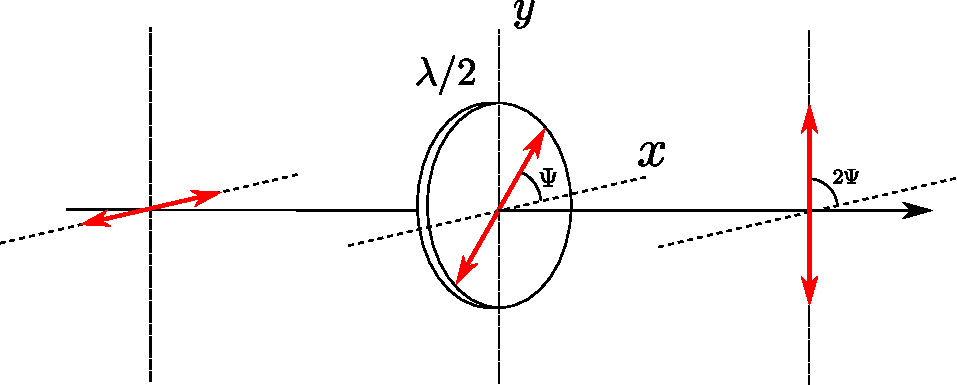
\includegraphics[scale=.7]{HWP_retarder}
\caption[Generación de estados de polarización lineales]{Propagación de un estado de polarización lineal horizontal a través de una placa de retardo de media onda
  vertical a $45^{\circ}$ que genera un estado de polarización lineal vertical. Las
placas de media onda introducen un retardo de fase de
$\pi$ radianes.}
\label{fig:hwp_retarder}
\end{figure}
Como en los casos anteriores, se puede representar la rotación de la
polarización usando el formalismo de Jones:
\begin{align*}
\mathbf{V} &=
R^{T}\left(\frac{\pi}{4}\right)\left(HWP\right)R\left(\frac{\pi}{4}\right)\mathbf{H},\\ 
\begin{pmatrix}
0\\1
\end{pmatrix}&=
 \frac{1}{\sqrt{2}}
\begin{pmatrix}
  1 &-1\\1&1
\end{pmatrix}
\begin{pmatrix} 1
  &0\\0&-1 \end{pmatrix}
 \frac{1}{\sqrt{2}}
\begin{pmatrix}
1&1\\-1&1
\end{pmatrix}
\begin{pmatrix}
1\\ 0
\end{pmatrix},
\\
&=
\begin{pmatrix}
0  & 1 \\1 & 0
\end{pmatrix}
\begin{pmatrix}
1\\ 0
\end{pmatrix},\\&=
\begin{pmatrix}
0\\1
\end{pmatrix}.
\end{align*}
Combinando rotadores ópticos (HWP) y retardadores de cuarto de onda (QWP),
podemos generar polarizaciones elípticas con cualquier inclinación y
elipticidad. Esto será de utilidad más adelante pues los autovectores
de las matrices de Jones indican los estados de polarización para los
cuales el sistema es transparente, es decir, no se modifica el vector
tras la operación de la matriz,
\[\mathbf{M}J_{\lambda} = \lambda J_{\lambda}.\]
Cuando se desea modulación de sólo fase en un SLM lo que se busca es
precisamente que no se modifique la polarización y por ende la
amplitud. El problema de calibrar moduladores se reduce a encontrar la
matriz que define el LC y extraer sus autoestados tal y como dicen
Pezzanitti y Davis en \citepChGen{Pezzaniti1993,Davis1998,Davis2003}.
En la sección que sigue se construirá un modelo para describir el
comportamiento de un cristal líquido enroscado (TN-LCD) en términos de
matrices de Jones.

\subsection{Propiedades ópticas de los cristales líquidos nemáticos enroscados (TN-LCD)}
\label{sec:Propiedades_opticas_de_TNLCD}
Los cristales líquidos del tipo TN-LCD son medios ópticos inhomogeneos
y anisotrópicos que localmente actúan como si fueran cristales
birrefringentes uniaxiales con su eje óptico orientado en la dirección
preferente de las moléculas. Como se mencionó en la sección
\ref{sec:LC-clasification} la anisotropía se debe a la forma obloide
de las moléculas del cristal, y en el caso de los TN la inhomogeneidad
viene dada por la orientación preferencial de las moléculas que es
función de su posición. Las propiedades ópticas se estudian suponiendo
que el material se puede representar como láminas delgadas perpendiculares a la
dirección de propagación, cada una de ellas actuando como si fuera un
cristal birrefringente uniaxial con su eje óptico rotado respecto al eje $x$ un ángulo
$\psi$ como se ilustra en la figura
\ref{fig:tn-lcd_sticks}.  
\begin{figure}[h!]
\centering
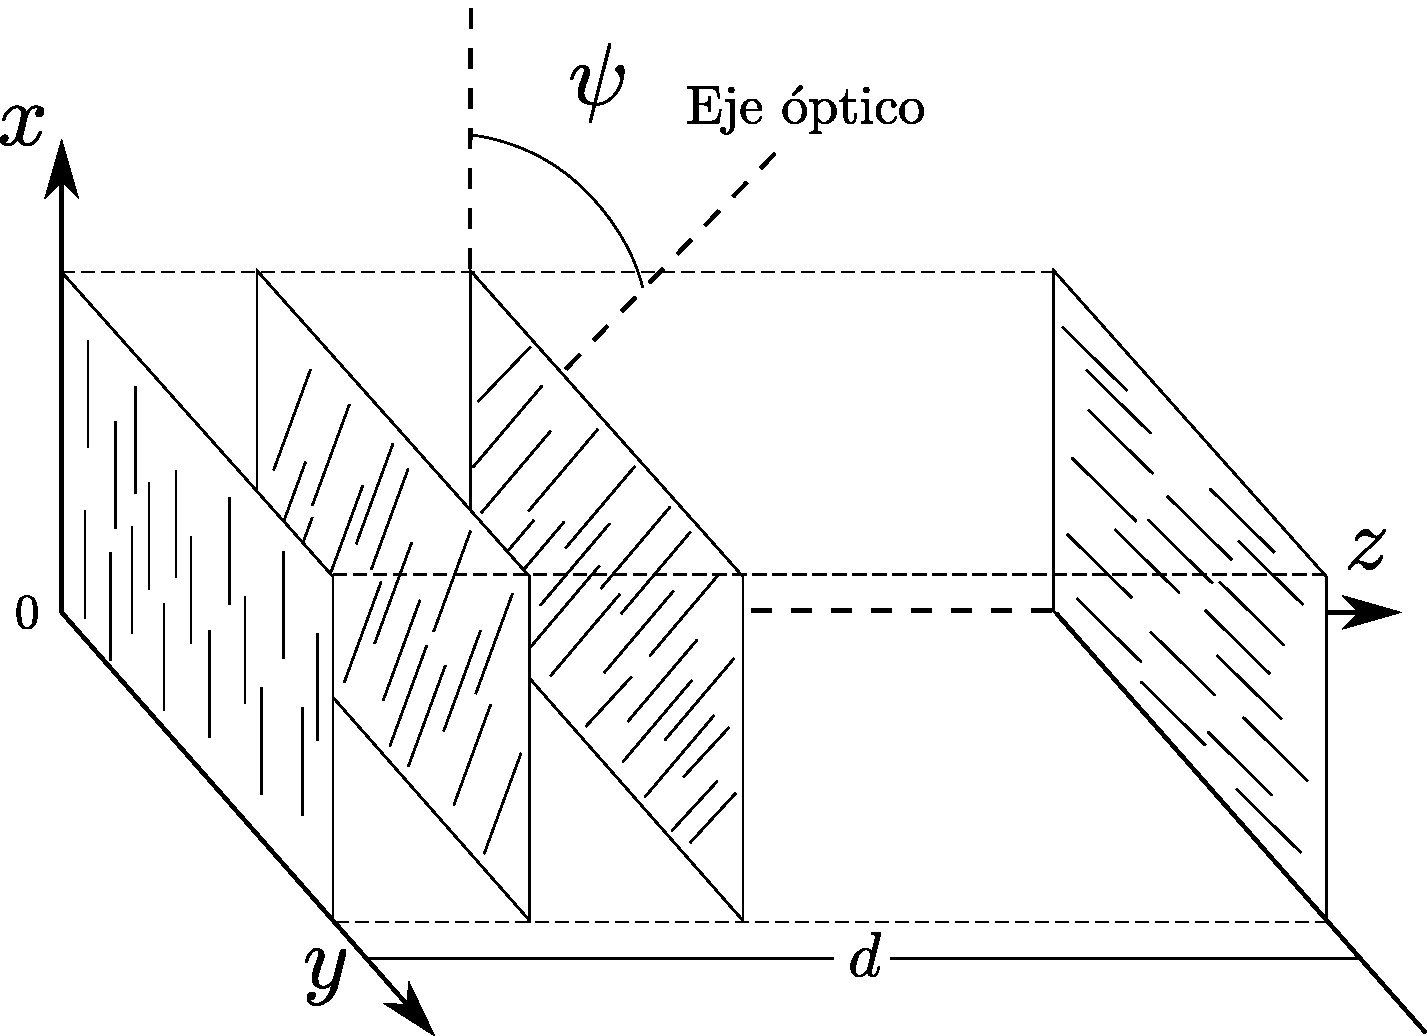
\includegraphics[scale = .3]{TN-LCD_sticks}
\caption[Propagación de la luz en un TN-LC]{Propagación de la luz en
  un cristal líquido del tipo Twisted 
  Nematic. En este diagrama el ángulo de entorchado es de $90^{\circ}$.}
\label{fig:tn-lcd_sticks}
\end{figure}
La rotación de cada \textit{lámina} de
moléculas se asume proporcional a la distancia desde la superficie de
entra da del LCD,
\begin{equation}
  \label{eq:twist_angle}
\psi(z)  =\alpha z.  
\end{equation}
Aquí la constante $\alpha$
se conoce como coeficiente de torsión, y el ángulo a la salida viene
dado por $$\phi \equiv \psi(d)=\alpha d.$$ Si se divide el cristal en
$N$ láminas, cada una tendrá un grosor $d/N$ y estará orientada en los ángulos
$\rho,2\rho,3\rho,\dots\left(N-1\right)\rho,N\rho$ con
$\rho=\phi/N$. Si cada lámina representa un cristal birrefringente, ésta tendrá una
birrefringencia asociada a su grosor dada por $$\beta_N = \frac{\pi
  d}{2N}\left(n_e-n_o\right).$$
La matriz de Jones general para el conjunto de todas las láminas se
encuentra como la multiplicación de cada una como se muestra a
continuación:
\[ M= W_NW_{N-1}\cdots W_3W_2W_1=\prod_{m=1}^NW_m = \prod_{m=1}^NR(m\rho)^TW_0R(m\rho), \]
dónde $R$ es la matriz de rotación, $W_m$ es la matriz de Jones para
el retardador $m$ rotada, y $W_0$ es aquella lámina en donde el eje rápido está
orientado con el eje $x$:
\begin{equation*}
W_0 =
\begin{pmatrix}
  e^{i\beta/2N} &0 \\ 0 & e^{-i\beta/2N} 
\end{pmatrix}.
\end{equation*}
Las matrices de rotación cumplen la siguiente regla:
\begin{align*}
R^T(\psi_m)R^T(\psi_{m-1}) &= R^T\left(\psi_m+\psi_{m-1}\right),\\
&=
\begin{pmatrix}
  \cos{\psi_m}&  -\sin{\psi_m}\\  \sin{\psi_m}&  \cos{\psi_m}
\end{pmatrix}
\begin{pmatrix}
  \cos{\psi_{m-1}}&  -\sin{\psi_{m-1}}\\  \sin{\psi_{m-1}}&  \cos{\psi_{m-1}}
\end{pmatrix},\\
&=
\begin{pmatrix}
  \cos{\psi_m}\cos{\psi_{m-1}}-\sin{\psi_m}\sin{\psi_{m-1}}&  
-(\cos{\psi_m}\sin{\psi_{m-1}}+\sin{\psi_m} \cos{\psi_{m-1}})\\
  \sin{\psi_m} \cos{\psi_{m-1}}+\cos{\psi_m}\sin{\psi_{m-1}}& 
 -\sin{\psi_m}\sin{\psi_{m-1}}+\cos{\psi_m}\cos{\psi_{m-1}}
\end{pmatrix},  \\
&=\begin{pmatrix}
  \cos{\left(\psi_m+\psi_{m-1}\right)}&  -\sin{\left(\psi_m+\psi_{m-1}\right)}\\
  \sin{\left(\psi_m+\psi_{m-1}\right)}&  \cos{\left(\psi_m+\psi_{m-1}\right)} 
\end{pmatrix}.
\end{align*}
Usando esto sobre las matrices de rotación, se puede realizar el
siguiente razonamiento, si $N=1$ entonces
\begin{equation*}
  M = R^T(\rho)W_0R(\rho).
\end{equation*}
Si en cambio $N=2$ se tiene
\begin{align*}
  M &= R^T(2\rho)W_0R(2\rho)R^T(\rho)W_0R(\rho),\\
      &=R^T(2\rho)W_0R(\rho)R(\rho)R^T(\rho)W_0R(\rho).
\end{align*}
Como $R(\rho)R^T(\rho)=\mathds{1}$ entonces
\begin{align*}
 M &= R^T(2\rho)W_0R(\rho)W_0R(\rho),\\
     &=R^T(2\rho)\left[W_0R(\rho)\right]^2.
\end{align*}
Y para $N=3$:
\begin{align*}
  M &= R^T(3\rho)W_0R(3\rho)R^T(2\rho)W_0R(2\rho)R^T(\rho)W_0R(\rho),\\
      &=R^T(3\rho)W_0R(3\rho)R^T(2\rho)\left[W_0R(\rho)\right]^2,\\
      &=R^T(3\rho)W_0R(\rho)R(2\rho)R^T(2\rho)\left[W_0R(\rho)\right]^2,\\
      &=R^T(3\rho)W_0R(\rho)\left[W_0R(\rho)\right]^2,\\
      &=R^T(3\rho)\left[W_0R(\rho)\right]^3.
\end{align*}
Ahora para una cantidad arbitraria $m$:
\begin{align*}
  M &= R^T(m\rho)W_0R(m\rho)R^T((m-1)\rho)\left[W_0R(\rho)\right]^{m-1},\\
      &=R^T(m\rho)W_0R(\rho)R((m-1)\rho)R^T((m-1)\rho)\left[W_0R(\rho)\right]^{m-1},\\  
      &=R^T(m\rho)W_0R(\rho)\left[W_0R(\rho)\right]^{m-1},\\
      &=R^T(m\rho)\left[W_0R(m\rho)\right]^{m}.
\end{align*}
Y así se obtiene la matriz general del TN-LCD según \citetChGen{Yariv2002} en
términos de dos matrices, una que cambia el estado de polarización y
otra que simplemente lo rota
\begin{align}
M&=R^T\left( \phi\right)
\left[W_0R\left(\frac{\phi}{N}\right)\right]^N,\\
&=R^T\left( \phi\right)
\begin{pmatrix}
  \cos{\frac{\phi}{N}e^{i\beta/N}} &  \sin{\frac{\phi}{N}e^{i\beta/N}}\\
  -\sin{\frac{\phi}{N}e^{-i\beta/N}} &  \cos{\frac{\phi}{N}e^{-i\beta/N}}  
\end{pmatrix}^N.
\label{eq:general_lcd_matrix}
\end{align}
La ecuación (\ref{eq:general_lcd_matrix}) puede ser simplificada aún
mas como muestran \citetChGen{Yeh1999} si se usa la identidad de Chebyshev
para matrices unimodulares  
\begin{equation}
  \begin{pmatrix}
    A & B \\ C & D
  \end{pmatrix}^m
=
\begin{pmatrix}
  \frac{A\sin{ (mZ) }-\sin(m-1)Z }{\sin{Z} }
  &\frac{B\sin{(mZ)}}{\sin{Z}}\\
\frac{C\sin{(mZ)}}{\sin{Z}}&   \frac{D\sin{ (mZ) }-\sin(m-1)Z }{\sin{Z} }
\end{pmatrix},
  \label{eq:chebyshev}
\end{equation}
con \[Z = \cos^{-1}{\left[\frac{1}{2}(A+D)\right]}.\]
Si se saca el límite cuando $(N\rightarrow \infty)$ se obtiene la
siguiente matriz
\begin{equation}
  \label{eq:TN-LCD_Jones_Matrix}
  M=
  \begin{pmatrix}
    \cos{\phi} & -\sin{\phi}\\\sin{\phi}&\cos{\phi}
  \end{pmatrix}
  \begin{pmatrix}
    \cos{\gamma}+i\beta\frac{\sin{\gamma}}{\gamma} & \phi\frac{\sin{\gamma}}{\gamma}\\
-\phi\frac{\sin{\gamma}}{\gamma}   & \cos{\gamma}-i\beta\frac{\sin{\gamma}}{\gamma}
  \end{pmatrix},
\end{equation} 
dónde:
\[\gamma=\sqrt{\phi^2+\beta^2}.\]

Ahora, la matriz de la ecuación (\ref{eq:TN-LCD_Jones_Matrix})  es la
matriz que todos los autores encontrados en el
estudio del estado del arte referencian y a partir de la cual se basan
para caracterizar moduladores. La matriz que representa un
SLM  tal como se estudió en esta sección es la forma más
simple de representar un cristal líquido del tipo twisted nematic y se
conoce como el modelo de \citetChGen{Saleh1990}. Este modelo
parte de asumir las siguientes aproximaciones:

\begin{itemize}
\item El TN-LCD se comporta como una sucesión de  láminas
  retardadoras en las cuales la orientación del vector director varía
  gradualmente desde un ángulo a la entrada hasta un ángulo a la
  salida y formando un ángulo de rotación conocido como twist angle. 
\item El ángulo de rotación (twist angle) es una función lineal
  proporcional a la profundidad en el cristal tal y como se expresa en
  la ecuación (\ref{eq:twist_angle}).
\item El ángulo de inclinación (tilt angle) se produce cuando se
  introduce un campo eléctrico que hace rotar las moléculas para
  alinearlas en su dirección. Éste ángulo se asume constante a lo
  largo del cristal para un voltaje específico. Si la birrefringencia
  es proporcional al ángulo de inclinación entonces al variar el
  voltaje ésta variará linealmente con respecto al voltaje.
\end{itemize}

En modelos posteriores como los de \citetChGen{Coy1996} y
\citetChGen{Marquez2000} se construyen matrices para el LCD que
corrigen comportamientos no lineales no previstos por  Lu y Saleh. El
principal factor a corregir en un LCD es la tendencia de las moléculas
cercanas a las paredes del cristal a conservar la dirección de pulido
de los vidrios que las contienen como se ilustra en la figura \ref{fig:lcd_models}.
\begin{figure}[h!]
\centering
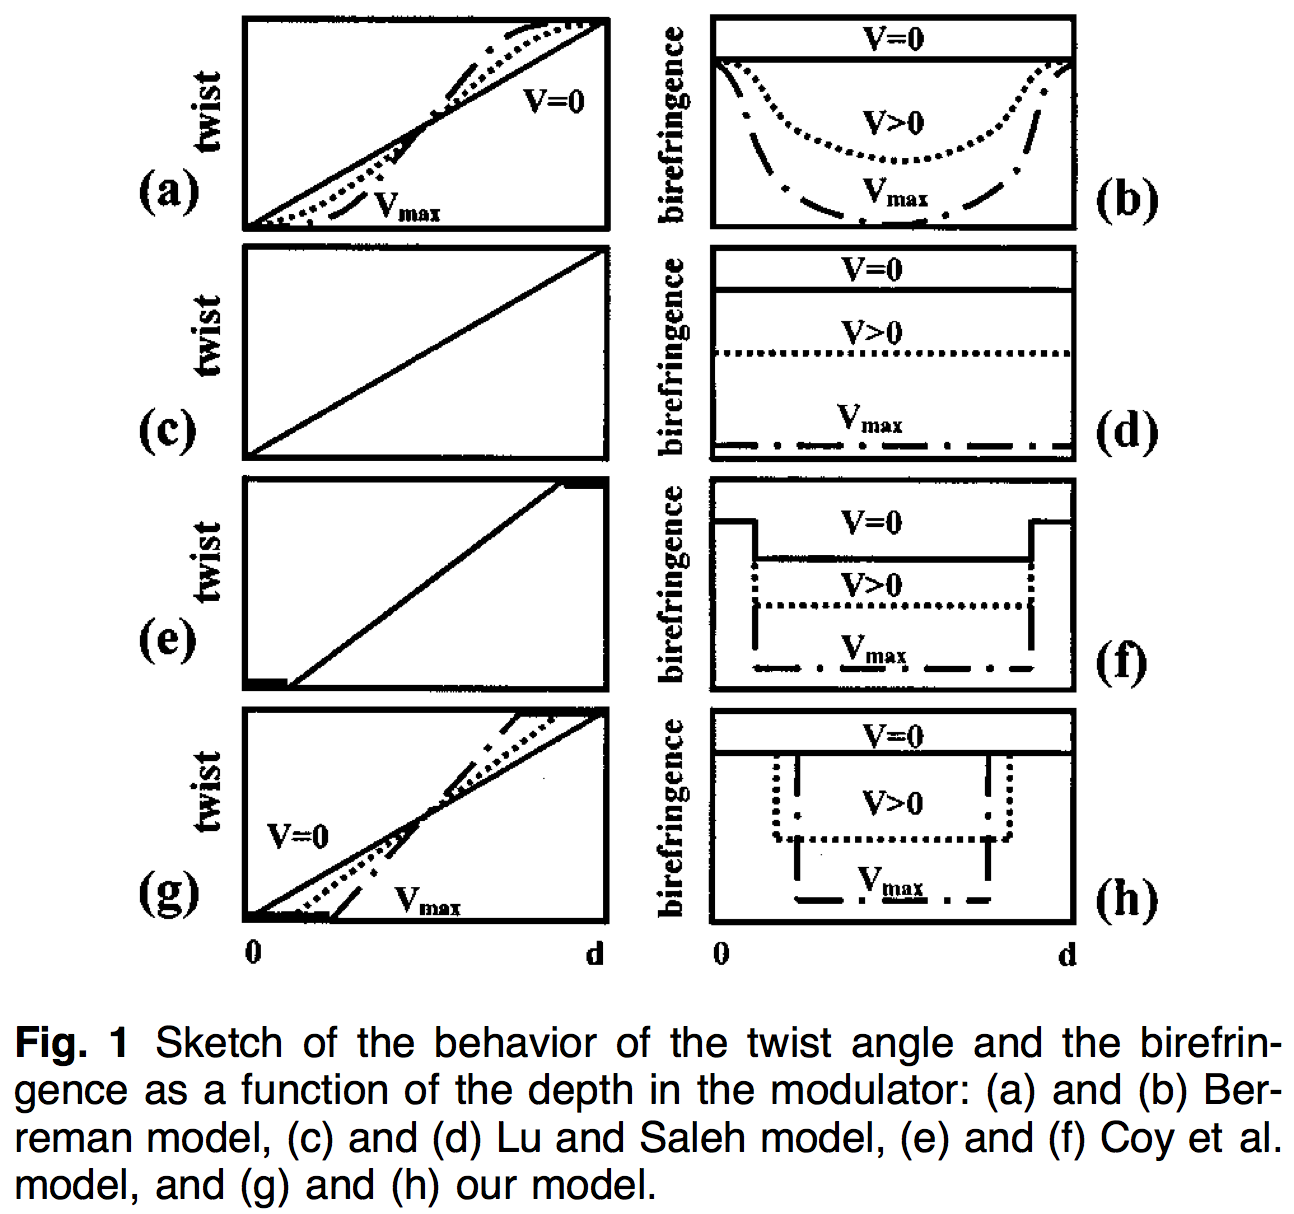
\includegraphics[scale=.5]{lcd_models}
\caption[Modelos de TN-LCD]{Modelos de TN-LCD tomado de \citetChGen{Marquez2000}.}
\label{fig:lcd_models}
\end{figure}
 Este efecto hace que el ángulo de
rotación no sea una función lineal  lo largo de la profundidad y que la
birrefringencia no sea una función lineal del voltaje.

\section{Revisión de la literatura}
Se realizó una revisión de la literatura en el contexto de calibración
de moduladores basados en TN-LCD y se encontró que para poder utilizar
una pantalla de cristal líquido como un modulador de sólo fase se debe
caracterizar el dispositivo como si fuera un elemento óptico que
afecta tanto la polarización como la fase de la luz. La mayoría de los
autores usan el cálculo de Jones para representar el efecto del SLM
sobre la luz como la operación de la matriz del SLM sobre un vector de
polarización a la entrada. Sin embargo, algunos autores como \citetChGen{Yu2012}, \citetChGen{Moreno2008} y Durán et al. \citepChGen{Duran2007} utilizan también
la medida de parámetros de  Stokes y matrices de Muller para obtener
curvas de calibración de los dispositivos. El reto en ambos casos es
encontrar una matriz que 
modele con precisión el comportamiento del modulador para diferentes
valores de voltaje aplicado. 

Hay dos formas básicas de caracterizar el
SLM, por una parte se puede seguir el camino riguroso y analizar el
TN-LCD desde el punto de vista físico como se hizo en la sección
anterior. Para este caso se deben encontrar los parámetros físicos que
determinan la matriz que se presentó en la fórmula
(\ref{eq:TN-LCD_Jones_Matrix}), es decir, la 
birrefringencia como función del voltaje, el ángulo de rotación de las
moléculas a la entrada del modulador, y el ángulo de rotación total
que experimentan las moléculas hasta la salida del modulador. Estos
parámetros son encontrados en la mayoría de los casos por medio de
ajuste de curvas con medidas experimentales de la tramitancia.  La
otra forma en la que se obtiene la matriz de Jones es asumiendo que el
sistema es como una caja negra que debe cumplir reglas menos
exigentes. En la figura \ref{fig:articulos_metodos} se ilustra por
medio de dos columnas la cantidad y fecha en las cuales se han
publicado artículos científicos en los cuales se usa uno u otro método
para caracterizar los moduladores. Adicionalmente se identificaron los
grupos que más han publicado sobre el tema. De la figura
\ref{fig:articulos_metodos} y de las fechas en los artículos de la
bibliografía se puede observar que la investigación en TN-LCD para
aplicación en procesamiento óptico tuvo su auge entre 1990 y 2010
aproximadamente, esto se debe como afirman \citetChGen{Kirsch1992}
a que a finales de los 80s las pantallas 
de LC para televisores portátiles resultaron interesantes a los
investigadores como dispositivos para generación dinámica de máscaras
de amplitud y fase. El declive en cambio, se debe a que los
moduladores de reflexión han ido reemplazando a los de transmisión por
 no necesitar de una caracterización y tener mejores prestaciones. 
También se ha concluido que los artículos que buscaban encontrar todos los
parámetros del modulador como el de \citetChGen{Marquez2000} y
el de \citetChGen{Zhisheng1998} en 1998 preceden en el tiempo a los artículos
donde se busca simplificar el modelo y asumir el comportamiento del
LCD como una caja negra, como los dos artículos de \citetChGen{Ma2010, Ma2011} en 2010 y
2011 o el de \citetChGen{Moreno2003} en 2003, que es en el cual nos
hemos inspirado para caracterizar nuestros SLMs. Los autores de esta
última referencia identificaron una necesidad de 
simplificar el proceso de caracterización, y entre sus argumentos 
están la simplicidad matemática y número reducido de medidas necesarias.
\begin{figure}[h!]
\centering
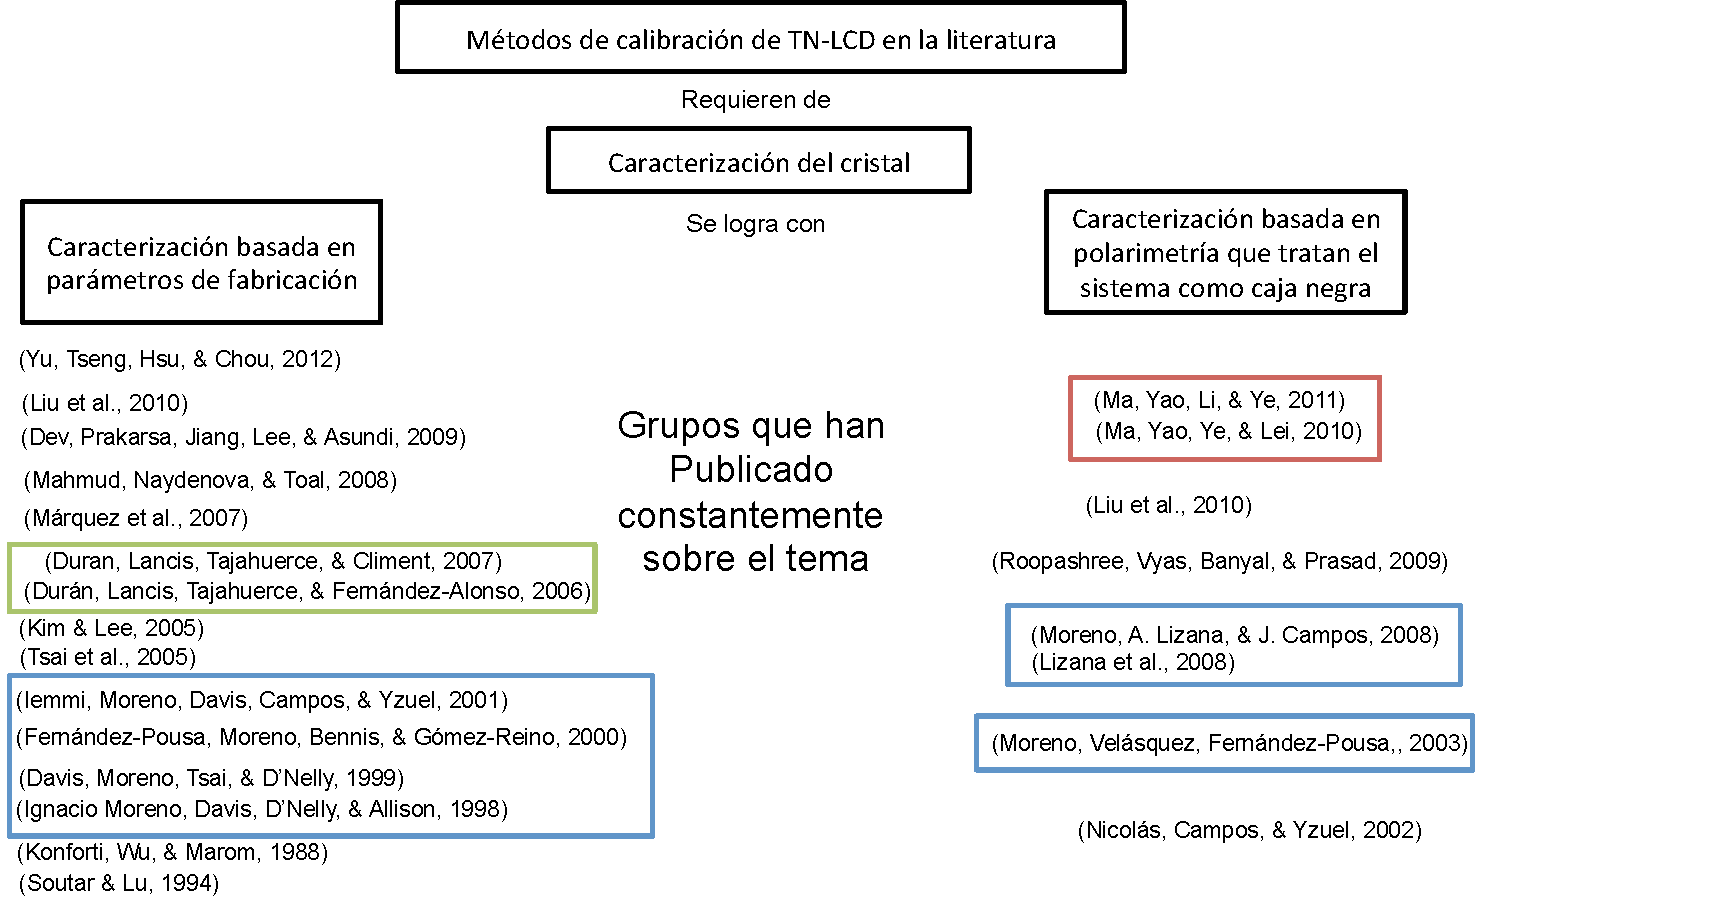
\includegraphics[scale=.6]{articulos_metodos}
\caption[Publicaciones en relación a la caracterización de TN-LCD]{Tabla de publicaciones en relación con caracterización de
  moduladores tipo TN-LCD. Los rectángulos representan los grupos que
  han publicado más en el tema y que resultan de mayor interés para
  este trabajo. }
\label{fig:articulos_metodos}
\end{figure}
El principal resultado del estudio del estado del arte fue encontrar
un patrón en la evolución del tema en la literatura desde los primeros
métodos para pantallas de televisor \citepChGen{Moreno1998} hasta campos
dónde se modula la polarización producidos por moduladores
\citepChGen{Moreno2011}. Este patrón tiene como columna vertebral al 
investigador Ignacio Moreno que, junto con otros investigadores en
universidades de España y California ha dirigido los avances en aplicaciones
científicas de pantallas TN-LCD. 

En lo que sigue de este capítulo presentaremos una variación del
método de caracterización \citetChGen{Moreno2003} implementada por nosotros y que
tambien considera el SLM como una caja negra. Esta implementación
involucró no solo análisis de datos sino también el diseño y
construcción de un sistema automatizado para la toma de medidas. 
Una vez caracterizado el SLM se
procedió a encontrar los autovalores de la matriz de Jones que
representan estados de polarización a la entrada y la salida del SLM 
que permiten una modulación de solo fase con la cual se pueden emular
elementos difractivos digitales tales como máscaras espiral de fase, prismas,
lentes de Fresnel e inclusive aberraciones. Los elementos difractivos producidos de forma
digital son la clave para producir haces Laguerre-Gauss.

\section{Caracterización de TN-SLM}
\label{sec:ChGV_Caracterizacion_de_SLM}
\lhead{Generación de Vórtices Ópticos: \textit{Caracterización de un TN-SLM}}

Como se mencionó antes, en la caracterización del SLM se pretende
encontrar estados de polarización a la entrada y salida del modulador
que produzcan modulaciones de solo fase, con buena tramitancia y con
un rango amplio de valores de fase. 
Por ende es necesario medir las modulaciones de amplitud y de fase. En
las siguientes secciones se muestra cómo medimos las modulaciones de
amplitud y fase. 

\subsection{Medida de la modulación de amplitud}
\label{sec:ChGV_med_mod_amp}

En la figura \ref{fig:PSG_PSD} se presenta un esquema del sistema
óptico usado para medir la modulación de amplitud. Si el haz tiene una
polarización lineal y se propaga en la dirección de $z$ la combinación
de un HWP y un primer QWP conocida como generador de estados de
polarización (PSG), permite producir estados de polarización
arbitrarios a la entrada del SLM. Luego, el haz llega al SLM y la modulación de amplitud se
da porque las moléculas de LC en el SLM cambian el estado de
polarización dependiendo del valor de voltaje aplicado. Cuando se añade un detector de estados de
polarización (PSD) compuesto por un segundo QWP y un polarizador, la amplitud del campo a la salida del polarizador
(P) dependerá de la matriz de Jones del SLM para el nivel de gris
actual y de los vectores de Jones asociados al PSG y PSD. A la salida
del PSD hay un estado con polarización lineal cuya intensidad puede
ser medida usando un fotodetector, o una cámara. 
 \begin{figure}[h!]
\centering
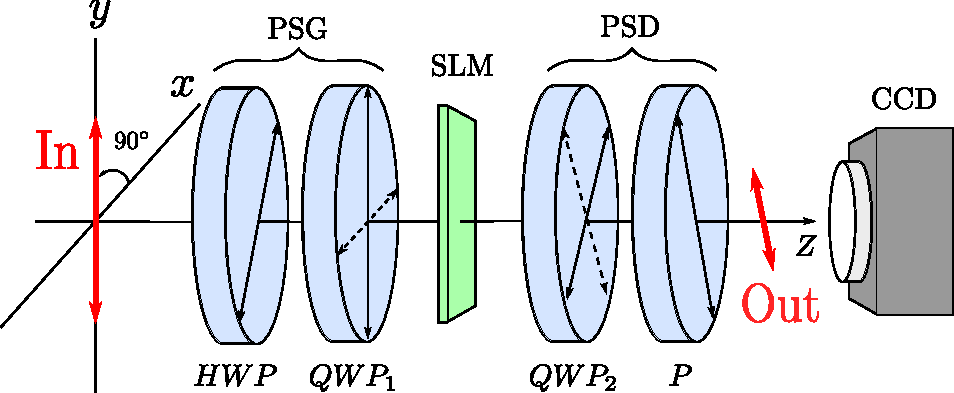
\includegraphics[scale=.8]{PSG_PSD.pdf}
\caption[Esquema de un sistema generador y analizador de estados de
polarización]{Esquema general de un sistema óptico para
  caracterización de modulación de intensidad de un TN-SLM.}
\label{fig:PSG_PSD}
\end{figure}

Desde el punto de vista matemático, el campo a la salida ($Out$) se puede
obtener multiplicando un vector de entrada $In$ por cada uno de
los elementos del sistema 
\begin{equation}
\label{eq:ChGV_Out}
Out = \left( \mathbf{P}\ \mathbf{QWP_2}\ \right) \mathbf{SLM}\ \left( \mathbf{QWP_1}\
\mathbf{HWP}\right)\ In.
\end{equation}
La intensidad medida por la cámara no es más que el módulo cuadrado de
este campo

\begin{equation}
I = |Out|^2 = Out^{\dagger}Out.
\end{equation}

A continuación, en la figura \ref{fig:amp_H_V_SLM_2002} se presenta
una curva de modulación de amplitud que se consigue graficando los
valores de intensidad normalizada cuando se varían los niveles de gris discretos
del SLM de 0 a 255. Como se mencionó antes, el nivel de gris es
proporcional al voltaje sobre las celdas de CL y corresponde a 0
cuando el ángulo de inclinación de las moléculas es de 90º con
respecto a la dirección de propagación. La
figura \ref{fig:amp_H_V_SLM_2002} es especialmente interesante porque
muestra el comportamiento del SLM marca Holoeye modelo LC2002 en la
configuración típica de pantallas LCD para royección, es decir, cuando
el PSG genera un estado de polarización a la entrada vertical y el
PSD detecta un estado horizontal. Como es de esperarse, en esta
configuración el SLM modula amplitud en un rango de 0 a 1 y con una
pendiente relativamente suave y lineal. 
\begin{figure}[h!]
\centering
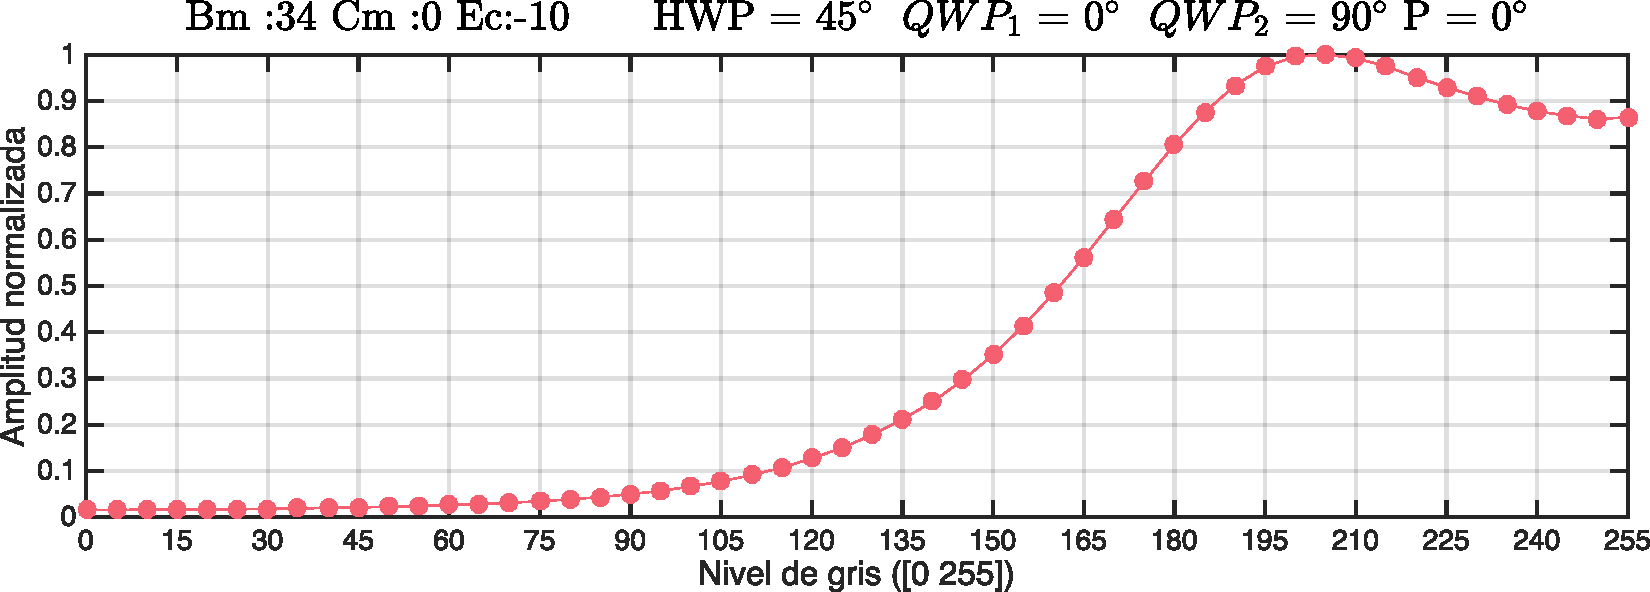
\includegraphics[scale=.55]{amp_H_V_SLM_2002.pdf}
\caption[Curva de modulación de amplitud para un estado no
óptimo]{Medida de la intensidad normalizada del SLM Holoeye LC-2002 en la configuración típica
  de pantallas LCD para royección. En este caso el PSG genera un estado de
  polarización a la entrada vertical y el PSD detecta un estado horizontal.}
\label{fig:amp_H_V_SLM_2002}
\end{figure}
Este tipo de modulaciónes
sirven para proyectar imágenes en niveles de gris y se pueden lograr
con dos polarizadores como PSG y PSD que generen estados líneales ortogonales
entre si.
% Como se explicó en la sección \ref{sec:Propiedades_opticas_de_TNLCD}
%  si el ángulo de torsión de las moléculas en el SLM es de $90^{\circ}$ y
% las moléculas a la entrada están alineadas con el eje horizontal, el
% estado de polarización a la salida será aproximadamente vertical.

No obstante, nuestro objetivo es encontrar una combinación de estados
de polarización que resulten en una baja modulación de amplitud y
buena tramitancia. 
\subsection{Medida de múltiples estados para alimentar un modelo de
  caja negra.}
\label{sec:ChGV_med_mod_amp}
La curva de la Fig. \ref{fig:amp_H_V_SLM_2002} caracteriza la modulación de amplitud del SLM para
una sola combinación de PSG y PSD. Una forma de buscar buenas
combinaciones de PSG y PSD consiste en plantear muchos estados
distintos y medir la modulación hasta encontrar un estado que produzca
los efectos deseados. Hacer esto experimentalmente es un proceso
engorroso y requiere de mucho tiempo porque hay muchas combinaciones
posibles que implican rotar elementos ópticos de forma precisa y con
alta repetibilidad. 
En cambio, vamos a medir experimentalmente sólo 6 combinaciones de PSG
y PSD propuestas por \citetChGen{Ma2010} y con
ellas alimentaremos un modelo de caja negra en el cual la matriz de
Jones para cada nivel de gris será encontrada por un método de ajuste
de parámetros.
% basado en un algoritmo de minimización basado en la búsqueda del
% gradiente. 
Una vez conocido el modelo del SLM se puede buscar el
estado que mejor satisface las condiciones de operación haciendo experimentos simulados con
los cuales sí es práctico hacer una búsqueda entre múltiples estados.

En esta sección se introducirá una notación alternativa para la
representación de estadodes de polarización, y se describiran los
estados ortogonales usados para la caracterización. 

\subsubsection{La notación de Dirac}

De forma similar a cómo sucede en la mecánica cuántica, los estados de
polarización arbitrarios generados por un PSG se pueden representar en
la notación de BraKets de Dirac como Ket's:
\begin{equation}
|J> = \begin{pmatrix} J_x \\ J_y\end{pmatrix} = \left( \mathbf{QWP_1}\
\mathbf{HWP}\right)\ In.
\end{equation}
Y siguiendo esta interpretación, el PSD correspondiente a un PSG dado
es el Bra, es decir, el vector que es complejo conjugado del Ket.
\begin{equation}
<J|= |J>^{\dagger} = \begin{pmatrix} J_x &  J_y\end{pmatrix} 
\end{equation}
Por otra parte, la matriz de Jones del SLM cumple el papel que tendría un
operador en la mecánica cuántica. Si los Bra y Ket representan vectores normalizados, la
intensidad del campo a la salida puede ser obtenida como el valor
esperado del operador del SLM cuando la base del PSG es proyectada
sobre la del PSD.
\begin{equation}
\label{eq:valor_esperado}
I = <J|\mathbf{SLM} |J> = 
\begin{pmatrix}
J_x & J_y
\end{pmatrix}
\begin{pmatrix}
A & B\\
 -B^* & A^* 
\end{pmatrix}
\begin{pmatrix}
J_x \\ J_y
\end{pmatrix}
,
\end{equation}
%donde $A$ y $B$ son números complejos.

La intensidad es una variable que se puede medir, y los vectores
correspondientes a los estados producidos por el PSG y el PSD son
conocidos. Encontrar los números complejos $A$ y $B$ para ensamblar la
matriz de Jones es un problema de polarimetría que requiere de
plantear un conjunto de medidas que den la información suficiente
sobre los cambios en polarización introducidos por el SLM. 
Tras implementar los métodos de caracterización basados en modelos de
caja negra, tanto de \citetChGen{Moreno2003} como de
\citetChGen{Ma2010}, y realizar nuestro propio método concluimos que
las siguientes 6 medidas de modulación son suficientes para una
correcta caracterización:
% Basandonos en el trabajo de Moreno, y con la convicción de que
% parametrizaban una variedad suficientemente diversa de situaciones
% escogimos las siguientes configuraciones de PSG y PSD para alimentar
% el algorítmo de ajuste.  
% \begin{align*}
% I_1 &= <\mathbf{V}|SLM|\mathbf{V}>& I_5 &=
%                                           <\mathbf{45^{\circ}}|SLM|\mathbf{45^{\circ}}>&I_9
%   &= <\mathbf{R}|SLM|\mathbf{R}>\\
% I_2 &= <\mathbf{H}|SLM|\mathbf{V}>&I_6 &=
%                                          <\mathbf{-45^{\circ}}|SLM|\mathbf{45^{\circ}}>&I_{10}
%   &= <\mathbf{L}|SLM|\mathbf{R}>\\
% I_3 &= <\mathbf{V}|SLM|\mathbf{H}>&I_7 &= <\mathbf{45^{\circ}}|SLM|\mathbf{-45^{\circ}}>&I_{11} &= <\mathbf{R}|SLM|\mathbf{L}>\\
% I_4 &= <\mathbf{H}|SLM|\mathbf{H}>&I_8 &=
%                                          <\mathbf{-45^{\circ}}|SLM|\mathbf{45^{\circ}}>&I_{12}
%   &= <\mathbf{L}|SLM|\mathbf{L}> 
% \end{align*}
\begin{align*}
I_1 &= <\mathbf{V}|SLM|\mathbf{V}>,& I_3 &=
                                          <\mathbf{45^{\circ}}|SLM|\mathbf{45^{\circ}}>,&I_5
  &= <\mathbf{CD}|SLM|\mathbf{CD}>,\\
I_2 &= <\mathbf{H}|SLM|\mathbf{V}>,&I_4 &=
                                         <\mathbf{-45^{\circ}}|SLM|\mathbf{45^{\circ}}>,&I_{6}
  &= <\mathbf{CI}|SLM|\mathbf{CD}>.
\end{align*}
Las curvas de modulación correspondientes a cada una de las medidas se
ilustran en la Fig \ref{fig:six_input_measures}. 
\begin{figure}[h!]
\centering
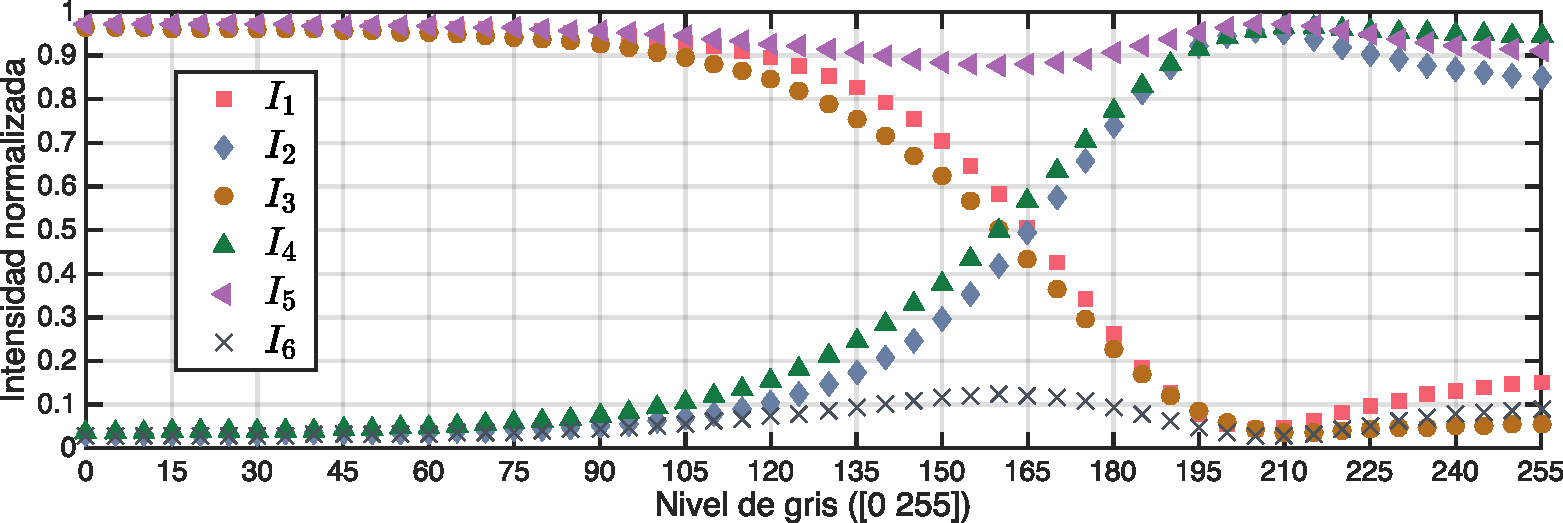
\includegraphics[scale=.55]{six_input_measures.pdf}
\caption[Curvas de modulación que sirven de entrada para el ajuste de
parámetros de la matriz de Jones del SLM]{Curvas de modulación que sirven de entrada para el ajuste de
parámetros de la matriz de Jones del SLM}
\label{fig:six_input_measures}
\end{figure}
Sólo con estas 6
curvas se observa que la modulación de amplitud es muy similar entre
polarizaciones lineales y que, como sería de esperarse, hay
complementariedad entre estados ortogonales.  Por otra parte, se
observa claramente que el SLM es transparente ante todo el rango de niveles cuando se genera y
detecta polarización circular derecha, y opaco cuando se genera
izquierda y se detecta derecha.

\subsubsection{Funcion a minimizar}

Una matriz de Jones que represente correctamente al SLM debe poder
emular al menos estas 6 medidas. Nosotros planteamos el siguiente
funcional a minimizar que actúa como una medida de la similitud entre
intensidades simuladas e intensidades adquiridas experimentalmente

\begin{equation}
\mathcal{L}(\mathbf{X,Y,Z,W}) = \sum_{ng=0}^{255}\sum_{i=1}^6 | I_{ng,i} -
<\mathbf{J_{i}}|\mathbf{SLM_{ng}}|\mathbf{J_{i}}>^2|.
\label{eq:ChGen_SLM_model_functional}  
\end{equation}
En la Eq. \ref{eq:ChGen_SLM_model_functional} el funcional consiste en
la suma de las diferencias cuadradas entre intensidades para cada
nivel de gris ($n$) y para cada combinación de PSG y PSD ($i$). Los
argumentos del funcional son vectores que representan el conjunto de números
reales $x_n, y_n, z_n, w_n$ que componen a los elementos complejos $A$ y $B$
de la matriz de Jones del SLM (ver 
Eq. \ref{eq:general_jones_matrix}) para un $n$ dado,
\begin{align*}
\mathbf{X} &= \sum_{n=0}^{255}x_n,&\mathbf{Y} &= \sum_{n=0}^{255}y_n,&\mathbf{Z} &= \sum_{n=0}^{255}z_n,&\mathbf{W} &= \sum_{n=0}^{255}w_n.
\end{align*} 
El funcional \ref{eq:ChGen_SLM_model_functional}  puede ser minimizado
variando los 1024 posibles valores 
de $X,Y,Z,W$ dentro del rango $-1:1$ en un algoritmo de
minimización. La minimización de los datos presentados en la
Fig. \ref{fig:six_input_measures} se llevo a cabo usando la función
 \href{http://goo.gl/tv5Iyz}{\bf{scipy.optimize.fmin\_l\_bfgs\_b}} del
 paquete de calculo científico \href{http://goo.gl/fRhz8s}{Scipy} del
 lenguaje de programación \href{https://www.python.org}{Python}. Ésta
 función conocida como \href{http://en.wikipedia.org/wiki/Limited-memory\_BFGS}{L-BFGS-B} implementa una versión de memoria limitada (L) del método quasi
 Newton conocido como Broyden-Fletcher-Goldfarb-Shano (BFGS) y permite
 la definición de condiciones de frontera (B) sobre los argumentos de
 entrada.  
La implementación en el lenguaje Python de la función a minimizar se muestra en el siguiente
recuadro, 
\begin{python}
def min_sq(x0,I_exp):
    """ Calculates squared differences for a minimization procedure.

    Given the experimental meassures of intensity and arbitrary values for 
    the parameters of an SLM Jones Matrix, this function gives a value to
    minimize. That value tells how close is the estimation of x, y, z, w 
    to the value that correctly models the SLM.

    :param x,y,z,w: Are a guess of real scalars that conform the Joung Matrix for the SLM.
    :param I_exp: Is a dictionary contanining intensities for every polarization state.
    """
    # brakets is a dictionary containing each pair of Jones vectors
    brakets = {1:translate_Ellipse_to_Jones([ 0,   0],      [0,0]),\
           2:translate_Ellipse_to_Jones([ pi/2,0],      [0,0]),\
           3:translate_Ellipse_to_Jones([ pi/4, 0],    [pi/4,0]),\
           4:translate_Ellipse_to_Jones([-pi/4, 0],    [pi/4,0]),\
           5:translate_Ellipse_to_Jones([pi/4,-pi/4],   [pi/4,-pi/4]),\
           6:translate_Ellipse_to_Jones([ -pi/4,pi/4],  [pi/4,-pi/4])}
    [x,y,z,w] = x0
    M = matrix([[ x + y*1j, z + w*1j],\
                [-z + w*1j, x - y*1j]])
    min_sum = 0
    I_sim = {}
    for i in range(1,nMeasures):
        Out, In = brakets[i]
        I_sim[i] = (In.H*M.H*Out * Out.H*M*In)
        min_sum += ((I_sim[i]-I_exp[i])**2)[0,0].real    
    return min_sum
\end{python}
\pagebreak
Y la llamada a la función de minimización se hace como se muestra a
continuación,\\

\begin{python}
bnds = ((-1, 1), (-1, 1),(-1, 1), (-1, 1))
cons = ({'type': 'eq', 'fun': lambda x:  x[0]**2+x[1]**2+x[2]**2+x[3]**2 - 1})
x,y,z,w = [0.0001, 0.0001, -0.0001, -0.0001] 
res_f = {}
for g in range(52):
    I_exp = I_list[g]
    res = fmin_l_bfgs_b(min_sq, [ x,y,z,w], fprime = None,\
                         approx_grad = 1,args = (I_exp,brakets),\
                         pgtol=1e-05, bounds =bnds)
    x,y,z,w = res[0]
    res_f[g] = res[0]
    print(res[0])
\end{python}
En este caso usamos un valor semilla para los valores de entrada muy
cercano a cero, utilizamos la opción de aproximación del gradiente
por medio de diferencias finitas y definimos la tolerancia de
convergencia como criterio de parada cuando el valor del funcional no
cambie a menos de $1e^{-5}$. Los detalles sobre las variables,
preprocesamiento, y los resultados se han subido a la red a un
repositorio de GitHub y se pueden observar en un la siguiente página
web \href{http://goo.gl/QQtcQX}{http://goo.gl/QQtcQX}.

En la figura \ref{fig:xyzw} se ilustran los valores de $X,Y,Z,W$ obtenidos luego de
ejecutar la minimización. 
\begin{figure}[h!]
\centering
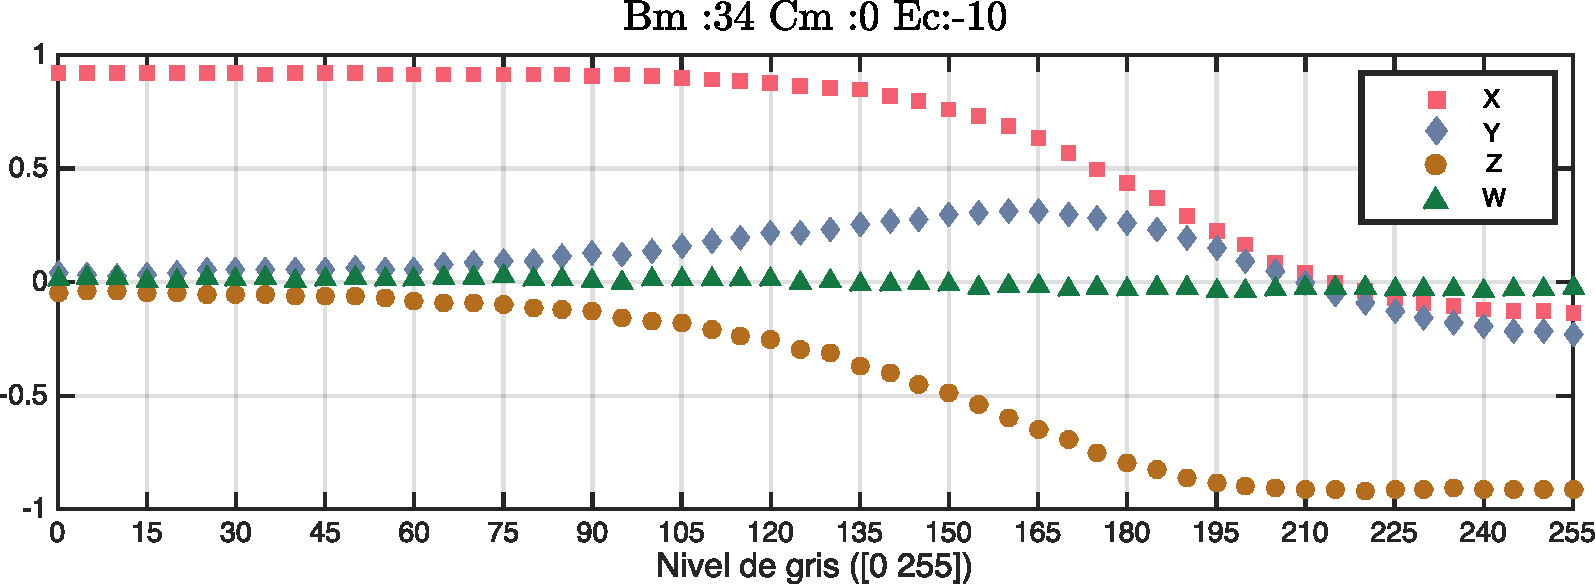
\includegraphics[scale=.55]{xyzw.pdf}
\caption[Parametros reales que conforman la matriz de Jones del SLM]{Parametros reales que conforman la matriz de Jones del SLM.}
\label{fig:xyzw}
\end{figure}
Estos valores , y en particular los de $X$ y
$Z$ siguen la misma tendencia que resultados de caracterizaciones
similares por \citetChGen{Moreno2003} y \citetChGen{Ma2010}, cosa que
da un primer indicio de un modelo adecuado. 
La siguiente sección trata la introducción de estados elípticos que
fueron planteados para corroborar la caracterización, y los resultados
experimentales obtenidos. 

\subsubsection{Comprobación experimental}

Con el fín de comprobar que la matriz obtenida era un modelo adecuado
del SLM se hicieron 100 medidas nuevas de modulación de amplitud y se
compararon con las simuladas por el SLM. En esas medidas se hicieron
todas las combinaciones posibles entre 10 vectores Ket y Bra usando la
numeración que se esquematiza en la Fig. \ref{fig:braket_100_notation}.
\begin{figure}[h!]
\centering
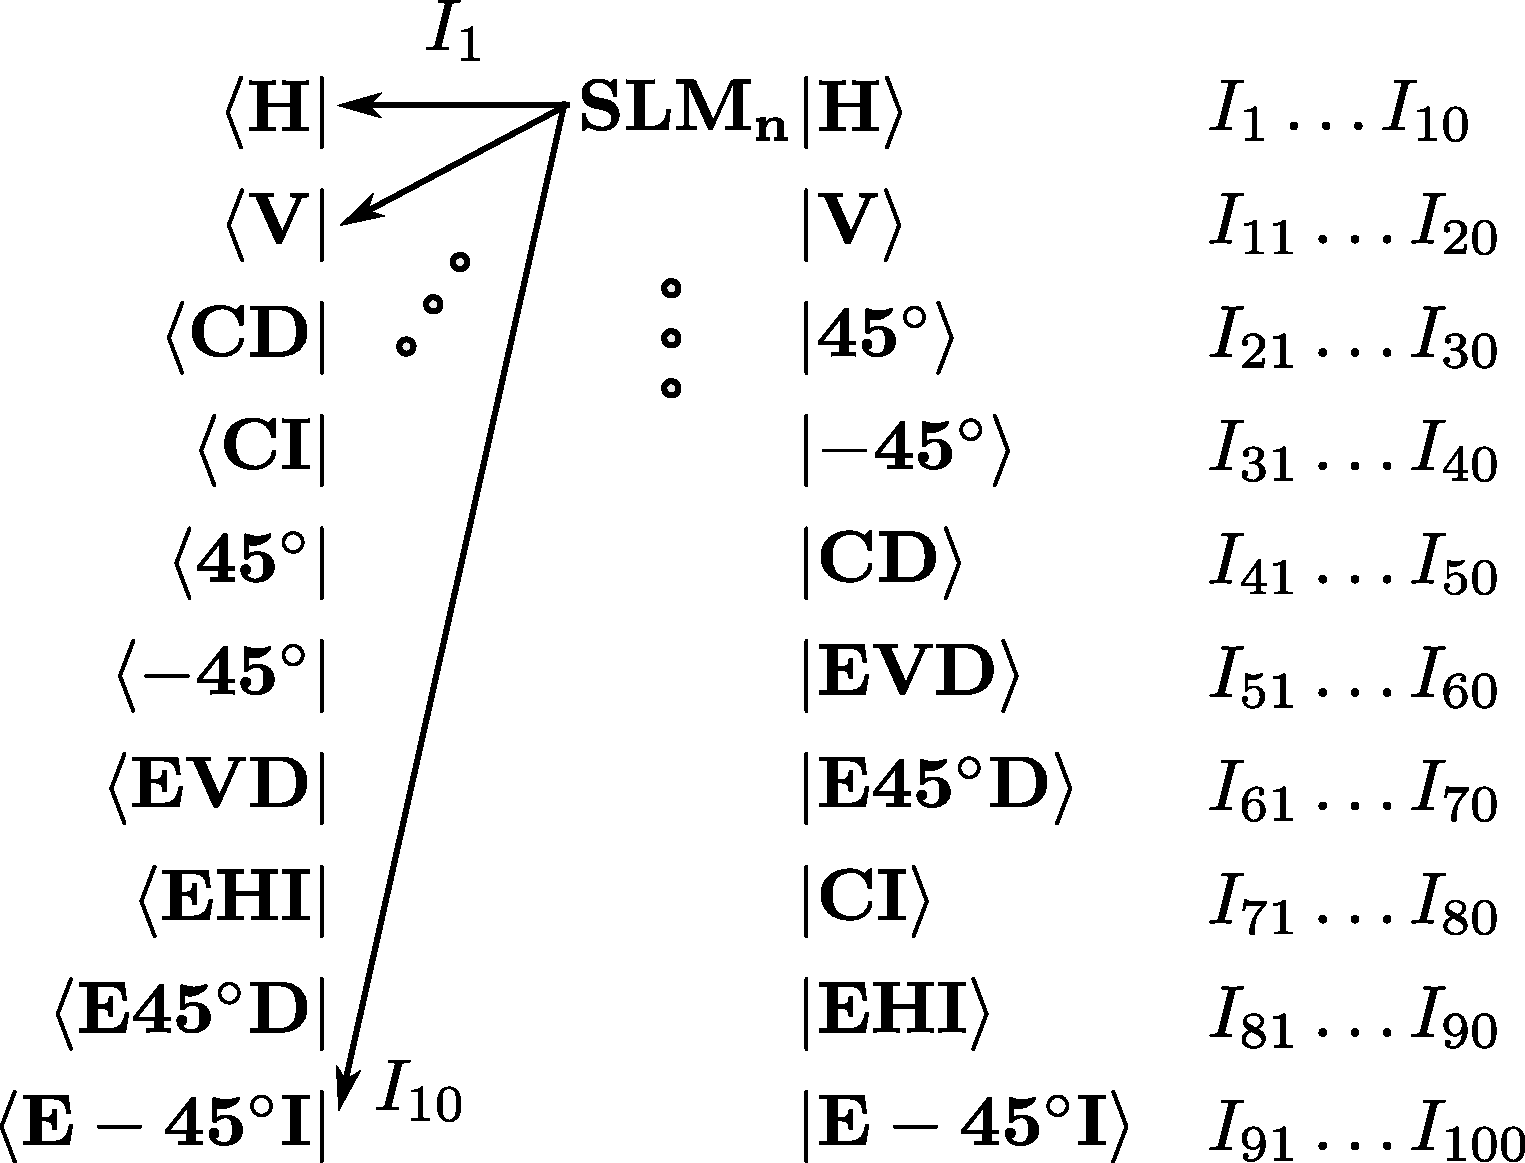
\includegraphics[scale=.4]{brakets.pdf}
\caption[Numeración de medidas experimentales de modulación para
corroboración del modelo de SLM]{Numeración de medidas experimentales de modulación para
corroboración del modelo del SLM. Por cada Ket hay 10 Bra y la
numeración se hace entre parejas en orden descendente con los pares
representados en la figura. }
\label{fig:braket_100_notation}
\end{figure}
Entre los estados usados se incluyeron dos parejas de estados
elípticos ortonormales no usados
como entrada del algorítmo de minimización. Los estados elípticos
corresponden a polarizaciónes elípticas horizontal, vertical, a
$45^{\circ}$ y a $-45^{\circ}$ con ángulo de elípticidad $\theta
=22.5^{\circ}$ como se muestra en la Fig. \ref{fig:elliptic_states}.
\begin{figure}
\centering
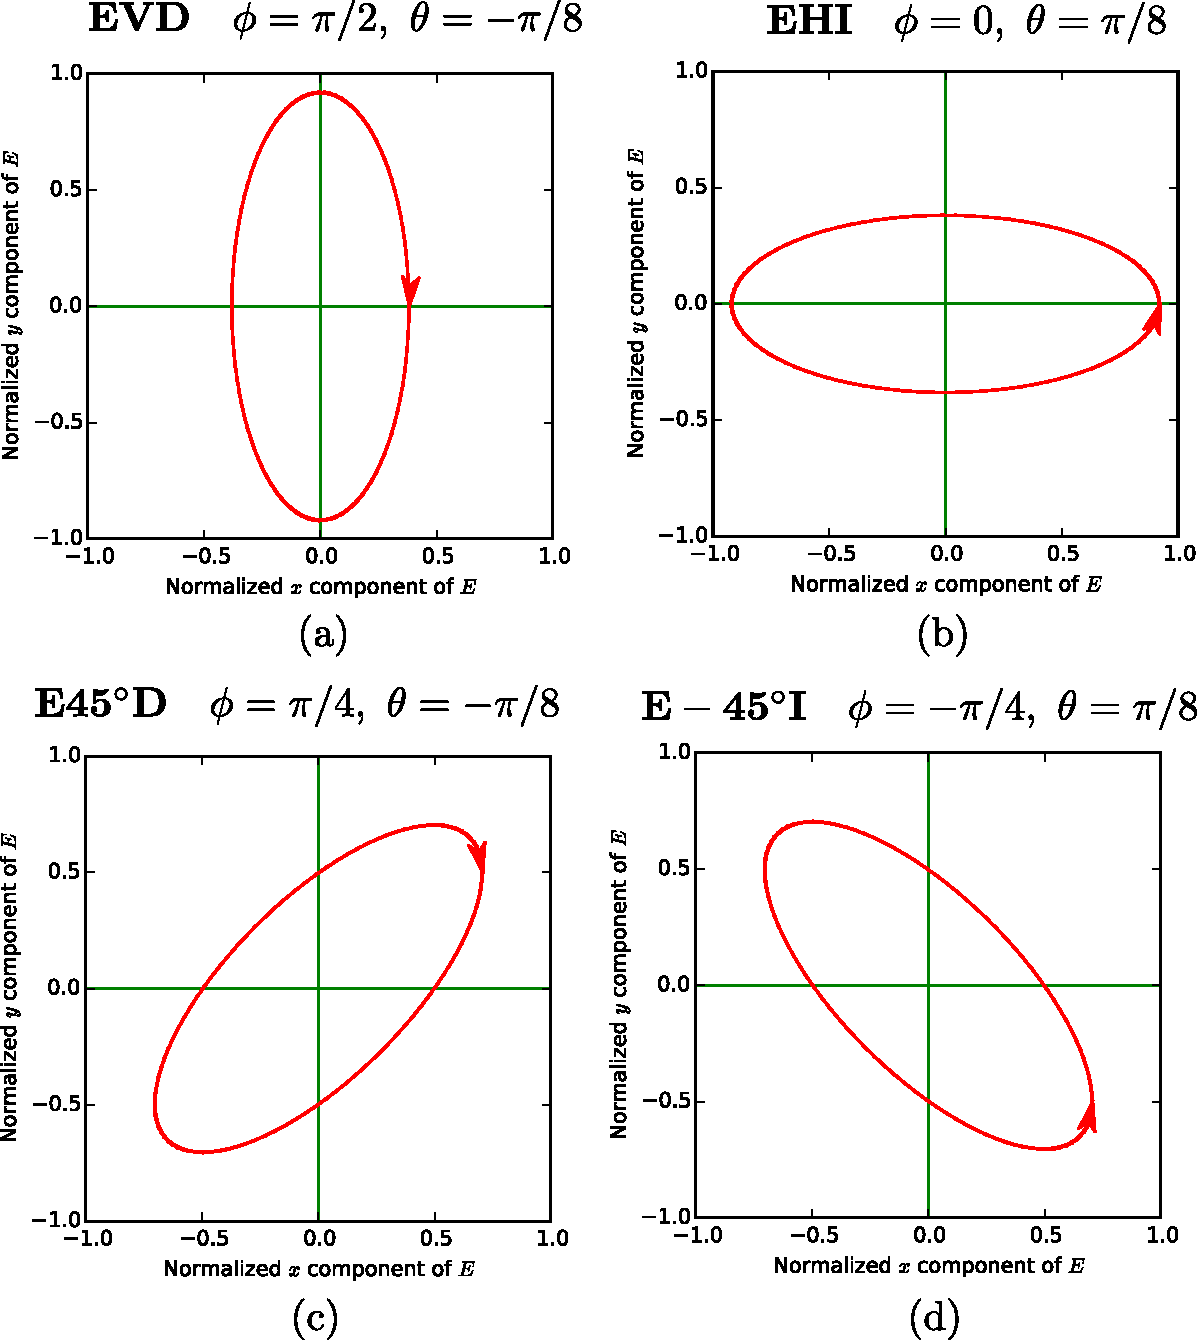
\includegraphics[scale = .6]{EVD_EHI_E45D_Em45I.pdf}
\caption[Estados de polarización elípticos]{Dos pares de estados de polarización
  elípticos ortonormales con ángulo de elipticidad $\theta = 22.5^{\circ}$. (a) Polarización Elíptica Vertical Derecha,
  (b) Elíptica Horizontal Izquierda, (c) Elíptica a $45^{\circ}$
  Derecha, y (d) Elíptica a $-45^{\circ}$ Izquierda.}
\label{fig:elliptic_states}
\end{figure}
Cuatro de los 100 resultados se muestran en la
Fig. \ref{fig:some_caracterization_results} y el resto se pueden
observar en la página web mencionada anteriormente \href{http://goo.gl/QQtcQX}{http://goo.gl/QQtcQX}. 
\newpage
\begin{figure}[h!]
\centering
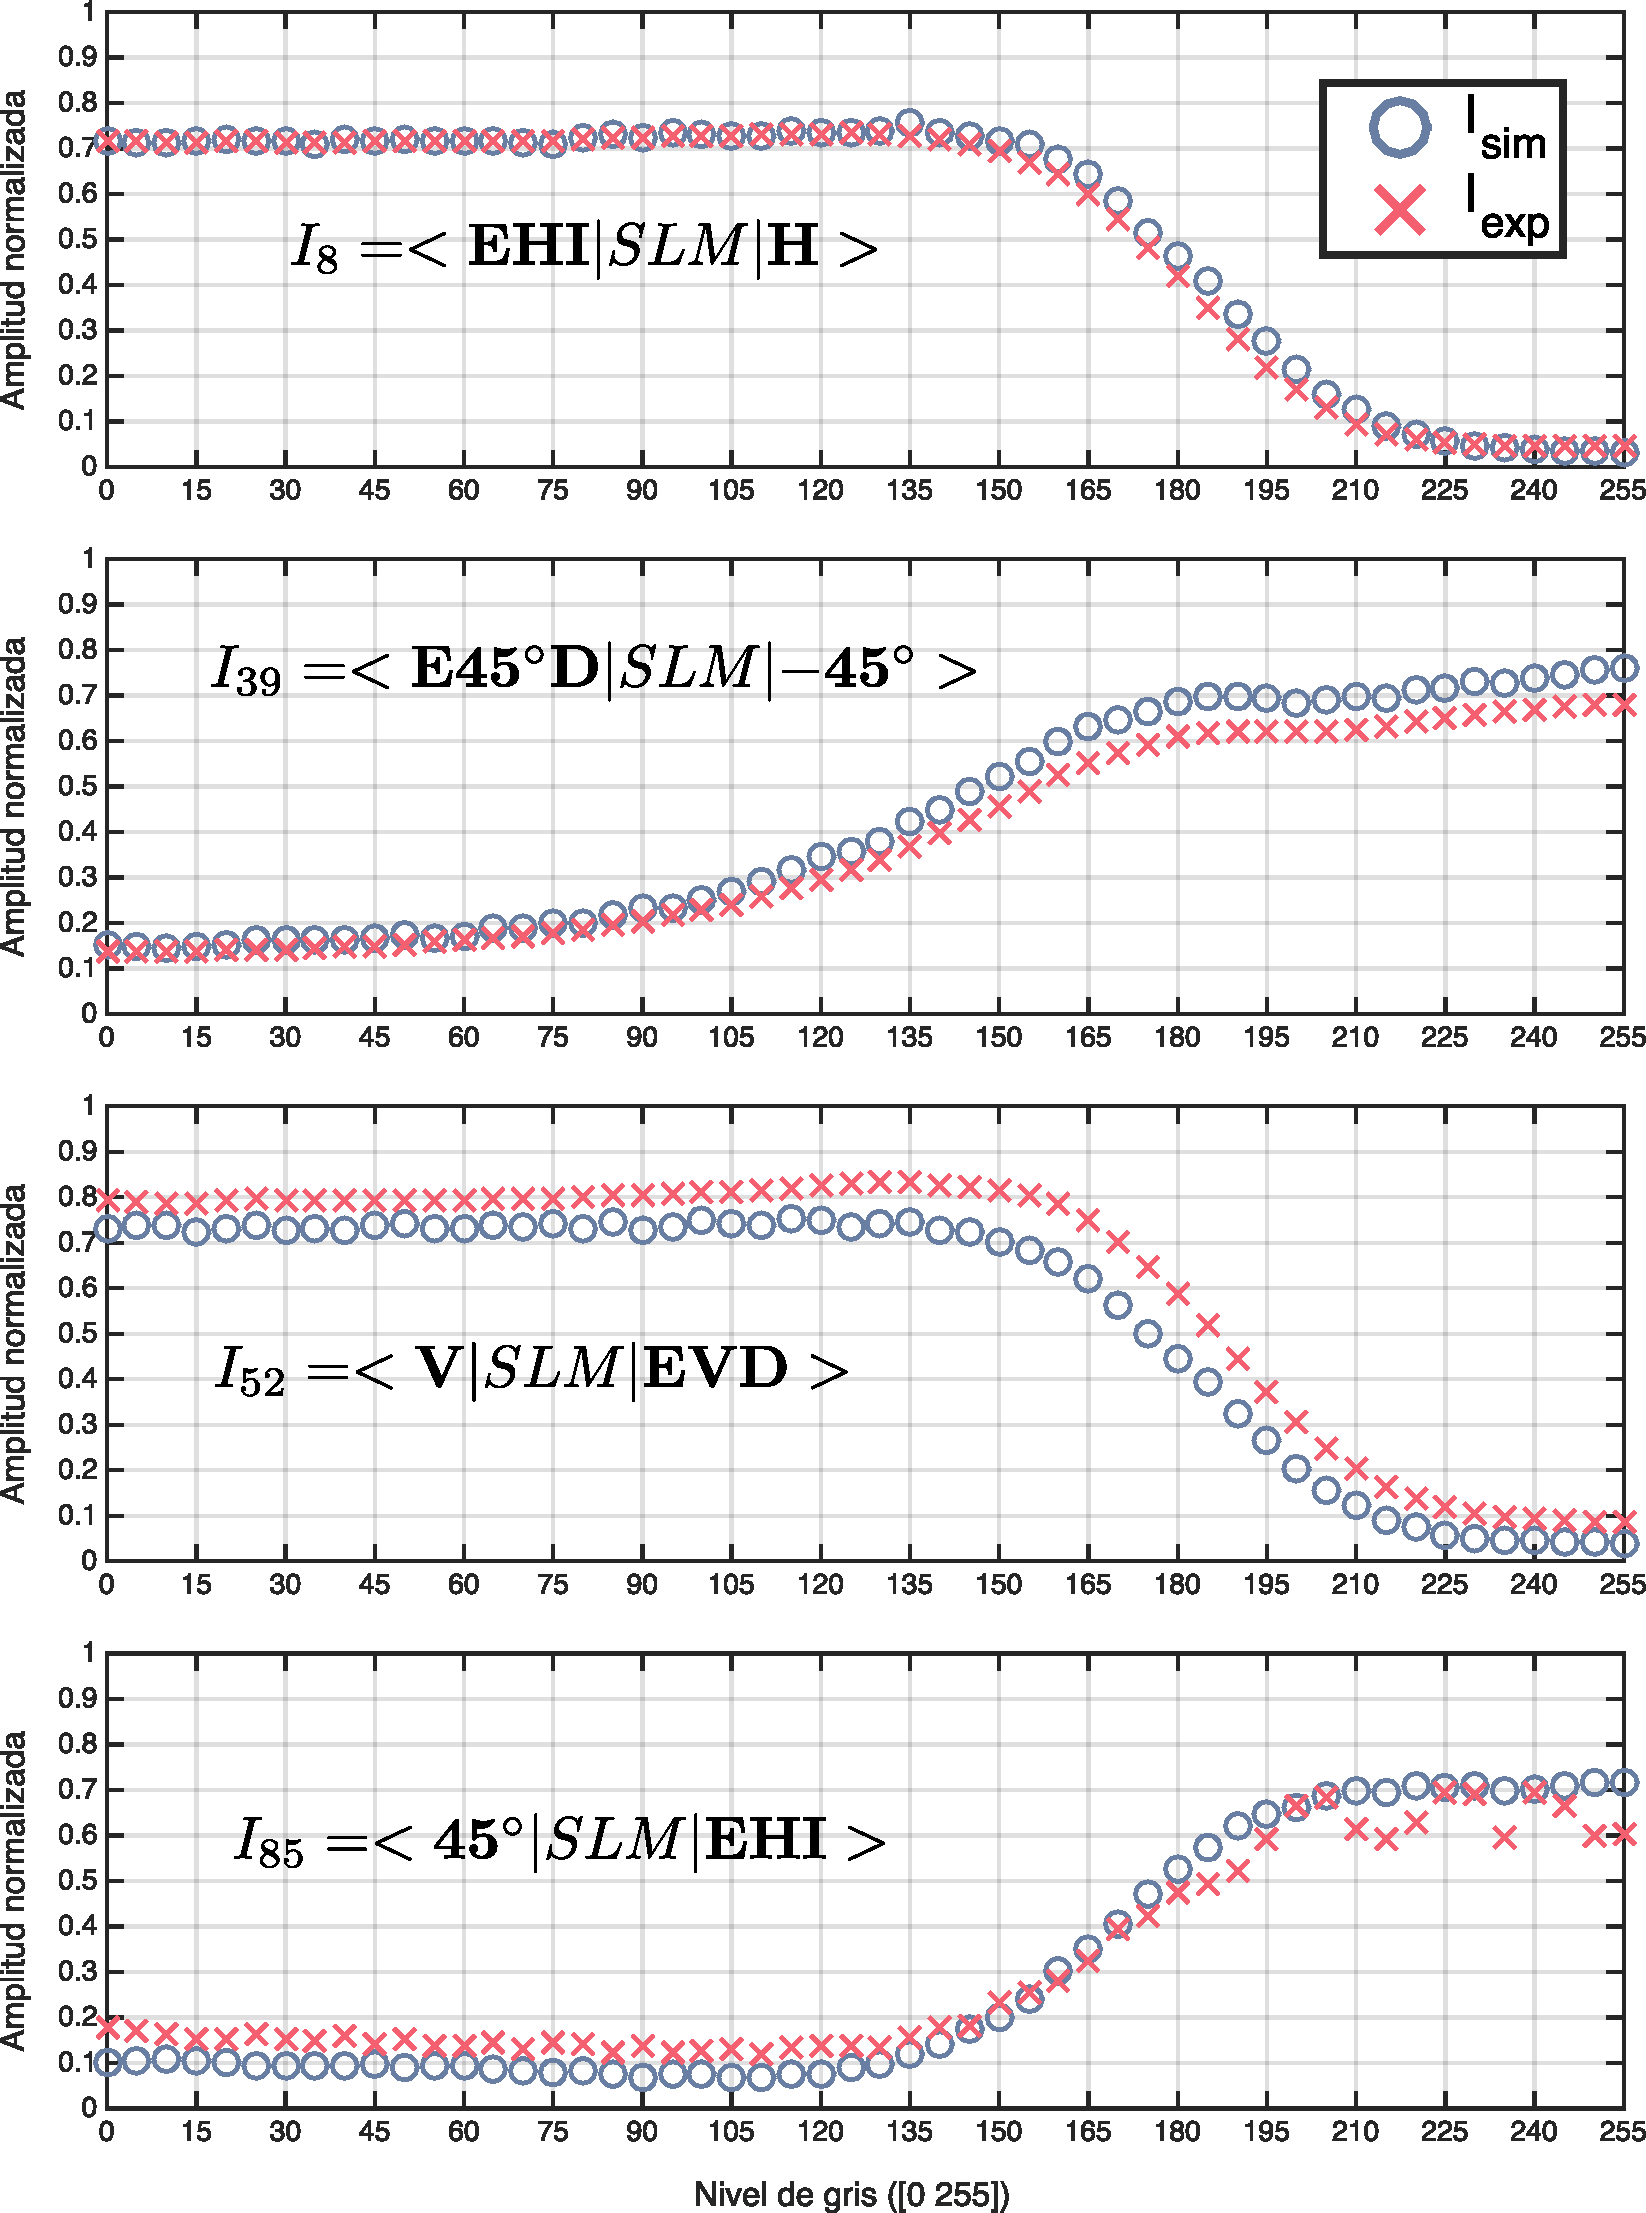
\includegraphics[scale=.5]{some_caracterization_results.pdf}
\caption[Curvas de modulación experimentales comparadas con las
simuladas usando el modelo obtenido]{Curvas de modulación
  experimentales de 4 de las 100 medidas comparadas con sus
  equivalentes simuladas usando la matriz recuperada por minimización.}
\label{fig:some_caracterization_results}
\end{figure}
Lo que muestran los resultados es que se logró una aproximación
excelente, y que el modelo de la matriz de Jones del SLM efectivamente
reproduce el comportamiento del elemento real. 

\begin{itemize}
\item Describir los dos algor[itmos que usamos para la reconstrucción
  de la modulación de fase y el de reconstrucción de modulación de
  amplitud. 
\item Describir el sistema de rotadores
\item Describir las aplicaciones para caracterización de motores
\item Describir el funcionamiento y la idea detrás de los programas de
  iPython para la detección de las matrices de Jones.
\item Describir la idea que tenemos para caracterizar LC utilizando
  interferometría.
\item mostrar los Vórtices obtenidos con buenas modulaciones y
  compararlos con los v[ortices que se obtenían antes.
\end{itemize}


\newpage
\pagebreak[4]
\bibliographystyleChGen{ezspanish}
\bibliographyChGen{References/Ch2}